\documentclass[11pt,a4paper]{article}

% Packages
\usepackage[utf8]{inputenc}
\usepackage[T1]{fontenc}
\usepackage{amsmath,amssymb}
\usepackage{geometry}
\geometry{margin=1in}
\usepackage{setspace}
\doublespacing
\usepackage{booktabs}
\usepackage{graphicx}
\usepackage{hyperref}
\hypersetup{colorlinks=true,linkcolor=blue,citecolor=blue,urlcolor=blue}
\usepackage{caption}
\usepackage{natbib}
\bibliographystyle{plainnat}
\usepackage{lineno}
\linenumbers
\usepackage{float}
\usepackage{array}
\usepackage{multirow}
\usepackage{threeparttable}

% Commands
\newcommand{\CosmicScanner}{\textsc{CosmicScanner}}
\newcommand{\G}{$\mathbf{G}$}
\newcommand{\V}{$\mathbf{V}$}
\newcommand{\etal}{\textit{et al.}}

\title{\bfseries\LARGE CosmicScanner: A Unified and Scalable Framework for Genome-Wide Association across Complex Trait Architectures}

\author{Jie Huang\\
  \small College of Animal Sciences, Zhejiang University, Hangzhou 310058, China\\
  \small \texttt{huangjie2025@zju.edu.cn}
}

\date{}

\begin{document}

\maketitle

\begin{abstract}
Modern genetic studies generate phenotypes that span continuous, longitudinal, repeated-measure, non-Gaussian, and multi-trait architectures, yet the GWAS software ecosystem remains fragmented: each model class is served by a different tool, with incompatible formats, GRM builders, and output schemas. Worse, the tools for repeated-measure and longitudinal data often construct record- or observation-level covariance matrices whose $O(n^3)$ factorization caps sample sizes well below biologically relevant scales. We present \CosmicScanner, a unified C++ framework that integrates \textbf{11 GWAS models} within a single engine sharing common genotype I/O, GRM construction, and null-model caching. Two algorithmic designs deliver scalability for the previously limiting model classes: (i) an \textbf{exact Woodbury subject-level reduction} that rewrites the repeatability-model covariance through the incidence matrix $\mathbf{Z}$, confining dense algebra to the subject level; and (ii) a \textbf{BLUP-based Kronecker multivariate LMM} that estimates Legendre random-regression coefficients first, then scans SNPs in coefficient space, sidestepping the observation-level covariance entirely. \CosmicScanner{} natively reads PLINK 1.9, PLINK 2.0, and BGEN with memory-mapped, multi-threaded decompression. Across validation against \textbf{GEMMA, EMmvGWAS, RepeatABEL, GMA, and GMAT}, association statistics showed near-perfect agreement for single-trait, multivariate, and repeatability scans (Pearson $r > 0.99$), and close concordance for unbalanced longitudinal RRM ($r=0.951$ against GMAT). Repeatability GWAS ran \textbf{10--20$\times$ faster at $\sim$10$\times$ lower memory}, and longitudinal RRM ran \textbf{213$\times$ faster at 93$\times$ lower memory} than the corresponding reference implementations or observation-level paths. Six extended models (maternal, threshold, GxE, survival, Poisson PSR, binomial PSR) pass type-I error calibration ($\lambda_{\text{GC}} \approx 1.00$); the maternal model recovers simulated residual variance within $<6\%$ error. The release build passes a 10-test CTest suite covering compatibility smoke tests, external-reference routes, sparse REML, multi-VC null models, SPA, REGENIE, and input adaptation. \CosmicScanner{} thus offers a single, validated, and scalable framework for genome-wide association across diverse complex trait architectures.
\end{abstract}

\noindent\textbf{Keywords:} GWAS; linear mixed model; longitudinal traits; repeated measurements; multivariate analysis; random regression; Woodbury identity; genomic relationship matrix

\section*{Significance}
\label{sec:significance}

The complexity of modern phenotypic data---repeated records, longitudinal trajectories, non-Gaussian outcomes, and correlated multi-trait panels---currently forces geneticists to chain together specialized tools that disagree on basic statistical assumptions and cannot scale to realistic record counts. \CosmicScanner{} resolves this fragmentation by unifying 11 GWAS model classes in one engine. It introduces an exact Woodbury reduction for repeated measurements and a BLUP-based coefficient-space strategy for longitudinal random regression. The result is a tool that reproduces established implementations with high concordance while running one to two orders of magnitude faster and using an order of magnitude less memory on the model classes that previously did not scale well.

\newpage
\section{Introduction}
\label{sec:introduction}

Genome-wide association studies (GWAS) have become the dominant approach for identifying genetic variants underlying complex traits since the first successful application in 2005 \citep{visscher2017,manolio2009}. Over the past two decades, GWAS methodologies have progressively expanded beyond the standard single-trait linear mixed model (LMM) to address increasingly complex phenotypic architectures. In livestock and plant breeding programs, individuals are routinely phenotyped multiple times across growth stages, parities, or environments, generating longitudinal and repeated-measure data \citep{mrode2014,schaeffer2004}. In biomedical cohorts such as the UK Biobank, phenotypes span continuous, binary, count, ordinal, and time-to-event outcomes \citep{sudlow2015,bycroft2018,willer2014}. Multi-trait joint analyses exploit phenotypic and genetic correlations to boost statistical power and reveal pleiotropic architecture \citep{korte2012,zhou2014mv,berg2019}. These developments have motivated a proliferation of specialized GWAS tools, each designed for a specific model class.

The linear mixed model has served as the foundational framework for GWAS since the introduction of the genomic relationship matrix (GRM)-based method by Yang \etal{} \citep{yang2011gcta} and the efficient mixed-model association (EMMA) algorithm by Kang \etal{} \citep{kang2010}. Tools such as GEMMA \citep{zhou2012gemma}, GCTA \citep{yang2011gcta}, BOLT-LMM \citep{loh2015}, and REGENIE \citep{mbatchou2021} have enabled scalable single-trait and, in some cases, multi-trait GWAS. For repeated-measure data, RepeatABEL \citep{ronnegard2010} implements a record-level mixed model with additive genetic, permanent environmental, and residual variance components. For longitudinal traits, GMA \citep{yao2022} and GMAT \citep{zhang2020gmat} provide random regression model (RRM) approaches using Legendre polynomial basis functions. For ordinal traits, POLMM \citep{bi2020} extends the proportional odds model with a genomic kinship-based random effect. For multi-trait analysis, EMmvGWAS \citep{jiang2024} and the multivariate LMM in GEMMA \citep{zhou2014mv} enable joint testing of multiple phenotypes.

Despite these advances, three structural gaps remain in the GWAS software ecosystem.

\textbf{First, model coverage is fragmented.} No single tool implements the full spectrum of models required by a modern study. A livestock population with repeated records, correlated traits, and ordinal outcomes forces researchers to chain RepeatABEL, GEMMA, and POLMM, each with its own input format, GRM builder, variance-component algorithm, and output schema. The resulting pipelines harbor hidden inconsistencies in statistical assumptions and are difficult to reproduce.

\textbf{Second, repeated-measure and longitudinal GWAS do not scale.} RepeatABEL constructs a dense record-level covariance $\mathbf{V}$ and fully eigendecomposes it, incurring $O(n_{\text{records}}^3)$ time and $O(n_{\text{records}}^2)$ memory \citep{ronnegard2010}. For 1,000 genotyped subjects with 10 records each, this means factorizing a $10{,}000 \times 10{,}000$ matrix. Observation-level RRM approaches face the same wall: the covariance dimension equals the total observation count, which routinely reaches tens of thousands \citep{zhang2020gmat}. In practice, exact repeated-measure and longitudinal GWAS are confined to small datasets, and analysts resort to ad hoc subject-mean aggregation that discards within-subject information.

\textbf{Third, modern genotype formats are incompletely supported.} PLINK 2.0 (.pgen) and BGEN have become the de facto standards for biobank data thanks to dosage encoding and compression, yet many GWAS tools still accept only PLINK 1.9 (.bed), forcing lossy or storage-heavy format conversion.

To close these gaps, we developed \CosmicScanner, a unified high-performance GWAS framework that integrates 11 model classes within a single C++ engine. Its guiding principle is that diverse trait architectures should be served by model-specific statistical formulations while sharing a common computational substrate---genotype I/O, GRM construction, null-model caching, and block-wise SNP scanning---so that statistical assumptions stay consistent across models, redundant computation is eliminated, and a single interface accepts any phenotype type.

The main contributions of this work are:

\begin{enumerate}
\item \textbf{Unified model coverage.} Eleven GWAS model classes---single-trait LMM, multivariate LMM, repeatability, random regression, maternal effect, single-step GWAS (ssGWAS), threshold/probit, count/binomial PSR, ordinal PSR, survival Cox, and GxE reaction-norm---are implemented in one package with consistent input/output conventions.
\item \textbf{Woodbury subject-level reduction for repeatability GWAS.} The exact record-level mixed model is preserved analytically, but all dense matrix operations are reduced from the record level ($n_{\text{records}}^3$) to the subject level ($n_{\text{subjects}}^3$), yielding \textbf{10--20$\times$ speedup and $\sim$10$\times$ memory reduction} versus RepeatABEL with statistically identical results.
\item \textbf{BLUP-based Kronecker RRM for unbalanced longitudinal GWAS.} Subject-level Legendre coefficients are first estimated by BLUP; SNPs are then scanned in coefficient space under a Kronecker covariance, bypassing the observation-level matrix entirely. On the GMAT benchmark this delivers \textbf{213$\times$ speedup and 93$\times$ memory reduction}.
\item \textbf{Comprehensive validation.} Association statistics show near-perfect concordance with GEMMA, EMmvGWAS, RepeatABEL, and GMA (Pearson $r > 0.99$) and close concordance with GMAT for unbalanced longitudinal RRM (Pearson $r = 0.951$, Spearman $\rho = 0.940$, top SNP concordant). An additional six extended models (maternal, threshold, GxE, survival, Poisson PSR, binomial PSR) pass type-I error calibration ($\lambda_{\text{GC}} \approx 1.00$); the maternal model additionally recovers known simulated residual variance within $<6\%$ error.
\end{enumerate}

\newpage
\section{Materials and Methods}
\label{sec:methods}

\subsection{Unified Data Input and GRM Construction}

\subsubsection{Genotype format support}

\CosmicScanner{} natively supports three genotype formats without external conversion:

\begin{itemize}
\item \textbf{PLINK 1.9} (.bed/.bim/.fam): The traditional binary format widely used in genetics research.
\item \textbf{PLINK 2.0} (.pgen/.pvar/.psam): The next-generation format supporting dosage-based encoding and efficient compression, designed for million-sample-scale biobank data.
\item \textbf{BGEN} (.bgen/.sample): The Oxford format used by the UK Biobank and other large cohorts, supporting probabilistic genotype calls.
\end{itemize}

All three formats share a common reader interface that provides genotype dosage vectors to the GWAS scanning engine. For PLINK 2.0 and BGEN, \CosmicScanner{} employs memory-mapped file I/O (mmap) combined with multi-threaded decompression to minimize memory overhead and maximize read throughput. Genotype dosages are loaded in blocks during SNP scanning to maintain a bounded memory footprint regardless of the total variant count.

\subsubsection{GRM construction}

The genomic relationship matrix (GRM) is constructed using the VanRaden (2008) method \citep{vanraden2008}:

\begin{equation}
\mathbf{G} = \frac{(\mathbf{M} - \mathbf{P})(\mathbf{M} - \mathbf{P})'}{2 \sum_{i=1}^{m} p_i (1 - p_i)}
\label{eq:grm}
\end{equation}

where $\mathbf{M}$ is the $n \times m$ genotype matrix coded as 0/1/2 reference-allele counts, $\mathbf{P}$ is the $n \times m$ matrix of column means ($2p_i$ for SNP $i$ with reference-allele frequency $p_i$), and the denominator scales $\mathbf{G}$ to be analogous to the pedigree-based numerator relationship matrix.

\CosmicScanner{} implements six GRM construction paths that cover PLINK, PGEN, and BGEN inputs with optional chromosome-partitioned computation for LOCO analysis. GRM construction is parallelized using OpenMP, with AVX2/AVX-512 SIMD instructions accelerating the inner-loop genotype cross-product accumulation. Variant filtering via \texttt{--extract}/\texttt{--exclude} (SNP ID lists), \texttt{--chr} (chromosome), and \texttt{--from-bp}/\texttt{--to-bp} (genomic interval) is applied at both GRM construction and SNP scanning stages to ensure consistency.

\subsubsection{Phenotype and covariate input}

\CosmicScanner{} accepts standard PLINK-format phenotype files with missing values encoded as \texttt{NA} or \texttt{-9}. For longitudinal and repeated-measure models, long-format phenotype files are supported where each row represents a single observation record keyed by \texttt{FID IID TIME}. Quantitative covariates (\texttt{--qcovar}) and categorical covariates (\texttt{--covar}) are specified as separate files in PLINK format. An input adaptation layer provides automatic conversion from CSV/TSV/TXT formats to the prepared input schema.

\subsection{Single-Trait LMM GWAS}

\subsubsection{Model}

The standard single-trait linear mixed model for GWAS is:

\begin{equation}
\mathbf{y} = \mathbf{X}\boldsymbol{\beta} + \mathbf{Z}\mathbf{u} + \mathbf{e}
\label{eq:lmm}
\end{equation}

where $\mathbf{y}$ is the $n \times 1$ phenotype vector, $\mathbf{X}$ is the design matrix for fixed effects and covariates, $\boldsymbol{\beta}$ is the corresponding effect vector, $\mathbf{Z}$ is the incidence matrix (typically the identity for genotyped individuals), $\mathbf{u} \sim N(\mathbf{0}, \sigma_g^2 \mathbf{G})$ is the random polygenic effect, and $\mathbf{e} \sim N(\mathbf{0}, \sigma_e^2 \mathbf{I})$ is the residual. The marginal covariance is $\mathbf{V} = \sigma_g^2 \mathbf{G} + \sigma_e^2 \mathbf{I}$.

\subsubsection{Exact LMM scan}

For exact LMM scanning, \CosmicScanner{} performs eigendecomposition of the GRM: $\mathbf{G} = \mathbf{U}\mathbf{D}\mathbf{U}'$, where $\mathbf{D}$ is the diagonal matrix of eigenvalues and $\mathbf{U}$ is the matrix of eigenvectors. The phenotype, covariates, and genotype dosages are rotated into the eigenvector basis: $\tilde{\mathbf{y}} = \mathbf{U}'\mathbf{y}$, $\tilde{\mathbf{X}} = \mathbf{U}'\mathbf{X}$, $\tilde{\mathbf{x}}_j = \mathbf{U}'\mathbf{x}_j$. In this rotated space, the covariance becomes diagonal: $\tilde{\mathbf{V}} = \sigma_g^2 \mathbf{D} + \sigma_e^2 \mathbf{I}$, enabling $O(n)$ per-SNP evaluation via weighted least squares.

\subsubsection{Fast-LMM approximation and LOCO}

When the variance ratio $\delta = \sigma_g^2 / \sigma_e^2$ is fixed at the null-model estimate rather than re-estimated per SNP, the scan reduces to a sequence of generalized least squares evaluations with identical covariance structure. This ``fast-LMM'' mode \citep{lippert2011} significantly accelerates genome-wide scanning while maintaining near-equivalent statistical power for common variants.

To avoid proximal contamination---the inflation of test statistics for SNPs on the same chromosome as the associated variant due to the GRM capturing linkage signals---\CosmicScanner{} implements LOCO (Leave-One-Chromosome-Out) analysis \citep{yang2012cojo}. In LOCO mode, a chromosome-specific null model is estimated using a GRM that excludes all SNPs on the target chromosome.

\subsection{IDUL/AIDUL Null-Model Acceleration}
\label{sec:idul}

The null-model variance-ratio estimation in LMM GWAS requires finding $\eta = \sigma_g^2 / \sigma_e^2$ that maximizes the restricted log-likelihood. The standard Brent search evaluates the likelihood function iteratively, which can require 20--50 iterations. We developed the IDUL (Iterative Dispersion Update using Likelihood) family of Fisher-scoring-based solvers that operate in the eigendecomposition space.

After GRM eigendecomposition and data rotation, the log-likelihood as a function of $\eta$ depends only on the diagonal eigenvalue matrix $\mathbf{D}$ and the rotated phenotype $\tilde{\mathbf{y}}$. The Fisher scoring update for $\eta$ is:

\begin{equation}
\eta^{(t+1)} = \eta^{(t)} + \mathbf{I}(\eta^{(t)})^{-1} \frac{\partial \ell}{\partial \eta}\bigg|_{\eta^{(t)}}
\label{eq:idul}
\end{equation}

where $\mathbf{I}(\eta)$ is the Fisher information and $\frac{\partial \ell}{\partial \eta}$ is the score function. Both quantities can be computed in $O(n)$ time using the eigenvalues $\mathbf{D}$ and rotated data.

Three variants are implemented: (i) \textbf{IDUL}, the basic Fisher-scoring solver; (ii) \textbf{IDUL+}, which adds a monotone likelihood safeguard that reduces step size when the log-likelihood decreases; and (iii) \textbf{AIDUL} (Accelerated IDUL), which incorporates Anderson acceleration (window size = 5) to extrapolate from the history of previous iterates. When the iterative solvers fail to converge, \CosmicScanner{} automatically falls back to the Brent solver to guarantee a valid result.

\subsection{Multivariate LMM GWAS}

\subsubsection{Model}

The multivariate linear mixed model for $q$ traits is:

\begin{equation}
\mathbf{Y} = \mathbf{X}\mathbf{B} + \mathbf{Z}\mathbf{U} + \mathbf{E}
\label{eq:mlmm}
\end{equation}

where $\mathbf{Y}$ is the $n \times q$ phenotype matrix, $\mathbf{B}$ is the fixed-effect matrix, $\text{vec}(\mathbf{U}) \sim N(\mathbf{0}, \mathbf{K} \otimes \mathbf{G})$ with trait covariance matrix $\mathbf{K}$ ($q \times q$) and GRM $\mathbf{G}$, and $\text{vec}(\mathbf{E}) \sim N(\mathbf{0}, \mathbf{R} \otimes \mathbf{I})$ with residual covariance $\mathbf{R}$. The marginal covariance is $\mathbf{V} = \mathbf{K} \otimes \mathbf{G} + \mathbf{R} \otimes \mathbf{I}$.

\subsubsection{Five methods}

\CosmicScanner{} implements five multivariate GWAS methods: (1) \textbf{EMMV}, an EMmvGWAS-compatible path using the kinship-based transformation $\boldsymbol{\Lambda} = \mathbf{G}\mathbf{R}^{-1}$; (2) \textbf{GEMMA-full}, performing per-SNP variance-component refit; (3) \textbf{Hybrid}, a LOCO-aware adaptive two-stage method combining fast EMMV screening with selective GEMMA-full refinement; (4) \textbf{EB} (Empirical Bayes), applying summary-level shrinkage to multivariate SNP effects; and (5) the standard \textbf{GEMMA-compatible} Wald/LRT/Score tests.

The hybrid method selects refinement candidates using a union of three criteria: p-value threshold, top-$K$ ranking, and Score/Wald discrepancy trigger. It also supports an optional Score-only pre-pass audit to identify SNPs where the fast screening test and the full Score test disagree.

\subsection{Repeatability Model GWAS}
\label{sec:repeatability}

\subsubsection{Model}

For record $j$ of subject $i$, the repeatability GWAS null model is:

\begin{equation}
\mathbf{y} = \mathbf{X}\mathbf{b} + \mathbf{Z}\mathbf{u} + \mathbf{Z}\mathbf{p} + \mathbf{e}
\label{eq:repeat}
\end{equation}

\begin{equation}
\mathbf{u} \sim N(\mathbf{0}, \sigma_g^2 \mathbf{G}), \quad \mathbf{p} \sim N(\mathbf{0}, \sigma_{pe}^2 \mathbf{I}), \quad \mathbf{e} \sim N(\mathbf{0}, \sigma_e^2 \mathbf{W}^{-1})
\label{eq:repeat_var}
\end{equation}

where $\mathbf{G}$ is the subject-level GRM ($n_{\text{subj}} \times n_{\text{subj}}$), $\mathbf{Z}$ is the $n_{\text{records}} \times n_{\text{subj}}$ incidence matrix, $\mathbf{p}$ is the permanent environmental effect, and $\mathbf{W}$ is an optional diagonal matrix of record-specific residual weights. The marginal covariance is $\mathbf{V} = \mathbf{Z}\mathbf{K}\mathbf{Z}' + \mathbf{R}$ where $\mathbf{K} = \sigma_g^2 \mathbf{G} + \sigma_{pe}^2 \mathbf{I}$ and $\mathbf{R} = \sigma_e^2 \mathbf{W}^{-1}$.

\subsubsection{Woodbury subject-level reduction}

The key algorithmic innovation is the application of the Woodbury matrix identity to avoid explicit construction and factorization of the dense record-level matrix $\mathbf{V}$:

\begin{equation}
\mathbf{V}^{-1} = \mathbf{R}^{-1} - \mathbf{R}^{-1}\mathbf{Z}(\mathbf{K}^{-1} + \mathbf{Z}'\mathbf{R}^{-1}\mathbf{Z})^{-1}\mathbf{Z}'\mathbf{R}^{-1}
\label{eq:woodbury}
\end{equation}

The core matrix requiring dense factorization is therefore subject-level:

\begin{equation}
\mathbf{M} = \mathbf{K}^{-1} + \mathbf{Z}'\mathbf{R}^{-1}\mathbf{Z}
\label{eq:core_matrix}
\end{equation}

This changes the main covariance operation from record-level dense algebra ($n_{\text{records}} \times n_{\text{records}}$) to subject-level dense algebra ($n_{\text{subjects}} \times n_{\text{subjects}}$). The determinant is computed via the matrix determinant lemma:

\begin{equation}
\det(\mathbf{V}) = \det(\mathbf{R}) \cdot \det(\mathbf{K}) \cdot \det(\mathbf{M})
\label{eq:woodbury_det}
\end{equation}

\subsubsection{Four strategies}

\CosmicScanner{} implements four repeatability GWAS strategies: (1) \textbf{Exact}, the full Woodbury solver with subject-level factorization (default); (2) \textbf{Fast}, using weighted subject-level mean aggregation; (3) \textbf{STCG}, caching the subject-level GRM as a Float32 binary file for out-of-core computation; and (4) \textbf{Mixed precision}, constructing the record-level kernel in Float32 and promoting to Float64 for the final solve.

\subsection{Random Regression Model (RRM) GWAS}
\label{sec:rrm}

\subsubsection{Model}

For subject $i$ observed at time $t_{ij}$, the random regression model expresses the SNP effect as a function of time:

\begin{equation}
y_{ij} = \mathbf{x}_{ij}'\boldsymbol{\beta} + \sum_{k=0}^{K} \phi_k(t_{ij}) a_{ik} + e_{ij}
\label{eq:rrm}
\end{equation}

where $\phi_k(t)$ are basis functions (Legendre polynomials by default; B-spline optionally), $a_{ik}$ is the random regression coefficient for subject $i$ and basis $k$, and the genetic covariance is $\text{Cov}(a_k, a_l) = K_{kl} \mathbf{G}$, where $\mathbf{K}$ is the $(K+1) \times (K+1)$ genetic covariance matrix and $\mathbf{G}$ is the GRM.

\subsubsection{BLUP-based Kronecker RRM for unbalanced data}

For unbalanced longitudinal data where subjects have different observation time points, \CosmicScanner{} implements a BLUP-based approach that avoids constructing the observation-level covariance matrix:

\textbf{Step 1 (Individual BLUP):} For each subject, Legendre random regression coefficients $\hat{\mathbf{a}}_i = (\hat{a}_{i0}, \hat{a}_{i1}, \ldots, \hat{a}_{iK})'$ are estimated via BLUP.

\textbf{Step 2 (Kronecker multivariate LMM):} The BLUP coefficient matrix $\hat{\mathbf{A}}$ ($n \times (K+1)$) is treated as a multivariate phenotype, and a Kronecker-structured multivariate LMM scans SNPs:

\begin{equation}
\text{vec}(\hat{\mathbf{A}}) \sim N(\mathbf{0}, \mathbf{K}_0 \otimes \mathbf{G} + \mathbf{P}_0 \otimes \mathbf{I})
\label{eq:kronecker}
\end{equation}

where $\mathbf{K}_0$ and $\mathbf{P}_0$ are the genetic and permanent environmental covariance matrices of Legendre coefficients. This reduces the covariance dimension from $n_{\text{observations}} \times n_{\text{observations}}$ to $n \times n$ (subject-level).

\subsection{Non-Gaussian Trait GWAS}
\label{sec:non_gaussian}

For phenotypes that deviate from the normal distribution---binary, count, binomial, and ordinal traits---\CosmicScanner{} implements a penalized quasi-likelihood (PQL) framework termed PSR-GWAS (Pseudo-Score Random regression GWAS). The approach linearizes the generalized linear mixed model via a working variate and passes the working residual variance to the LMM scanner as observation weights.

For \textbf{binary traits}, a threshold (probit or logit) model is fitted with optional saddlepoint approximation (SPA) for case-control imbalance. For \textbf{count data}, a Poisson or binomial GLMM is fitted with an optional offset. For \textbf{ordinal traits} with $K$ ordered categories, a stacked proportional-odds model is implemented via the stacked PSR approach with dense-zkz representation and grid REML variance-component estimation. For \textbf{survival data}, a Cox proportional hazards model is fitted, and martingale residuals are used as the pseudo-phenotype.

\subsection{Maternal-Effect and Single-Step GWAS (ssGWAS)}
\label{sec:other_models}

For traits influenced by maternal effects, \CosmicScanner{} implements a multi-component variance model with direct additive, maternal additive, direct-maternal covariance, and maternal permanent environmental effects. For populations with incomplete genotyping, single-step GWAS (ssGWAS) integrates pedigree ($\mathbf{A}$) and genomic ($\mathbf{G}$) information via the combined relationship matrix $\mathbf{H}^{-1} = \mathbf{A}^{-1} + \text{diag}(\mathbf{0}, \mathbf{G}^{-1} - \mathbf{A}_{22}^{-1})$ for variance-component estimation, followed by a SNP-level Wald scan.

\subsection{GxE Reaction-Norm Model and Rare-Variant Tests}
\label{sec:gxe}

For gene-by-environment interaction analysis, \CosmicScanner{} models the SNP effect as a linear function of an environmental covariate $E$, performing a 2-df joint Wald test for the main and interaction effects \citep{ko2019}. For rare-variant association, SKAT and burden tests are implemented with beta-weight function and Davies' method for p-value computation \citep{zhou2022saigegene}.

For UK Biobank-scale data, a REGENIE-style two-step regression is available: Step 1 performs block-wise ridge regression with LOCO predictions, and Step 2 performs streaming single-SNP association tests after residualizing against covariates and the LOCO prediction.

\subsection{Implementation}
\label{sec:implementation}

\CosmicScanner{} is implemented in C++17 using the Eigen3 linear algebra library. Multi-threaded parallelization is achieved via OpenMP, with AVX2 and AVX-512 SIMD instructions where supported. The software follows a modular architecture with format-specific genotype readers, an LMM engine for null-model preparation and SNP scanning, model-specific implementations for each trait architecture, and a shared core library (libCosmicCore) for VCE, eigendecomposition, and matrix operations. The software is cross-platform (Linux native, Windows via WSL2) and is freely available at \url{https://github.com/huangjie2025/CosmicScanner} under the MIT License.

\newpage
\section{Results}
\label{sec:results}

We organized the validation into four threads that mirror the design goals of \CosmicScanner: (i) \textbf{statistical fidelity} to established reference tools, (ii) \textbf{format consistency} across PLINK/PGEN/BGEN, (iii) \textbf{scalability} on the model classes that previously did not scale, and (iv) \textbf{calibration} of the non-Gaussian PSR-GWAS extensions. Across the externally benchmarked model classes, \CosmicScanner{} reproduces reference implementations with near-perfect agreement for single-trait, multivariate, repeatability, and balanced RRM scans, and with close concordance for unbalanced longitudinal RRM. It simultaneously delivers one to two orders of magnitude improvements in runtime and memory on repeated-measure and longitudinal data. Figure~\ref{fig:architecture} provides an overview of the software architecture and model coverage; Table~\ref{tab:summary} summarizes the 11 models and their validation status; the subsections below detail the quantitative evidence with supporting Figures~\ref{fig:woodbury}--\ref{fig:rrm_dynamic}.

\begin{figure}[H]
  \centering
  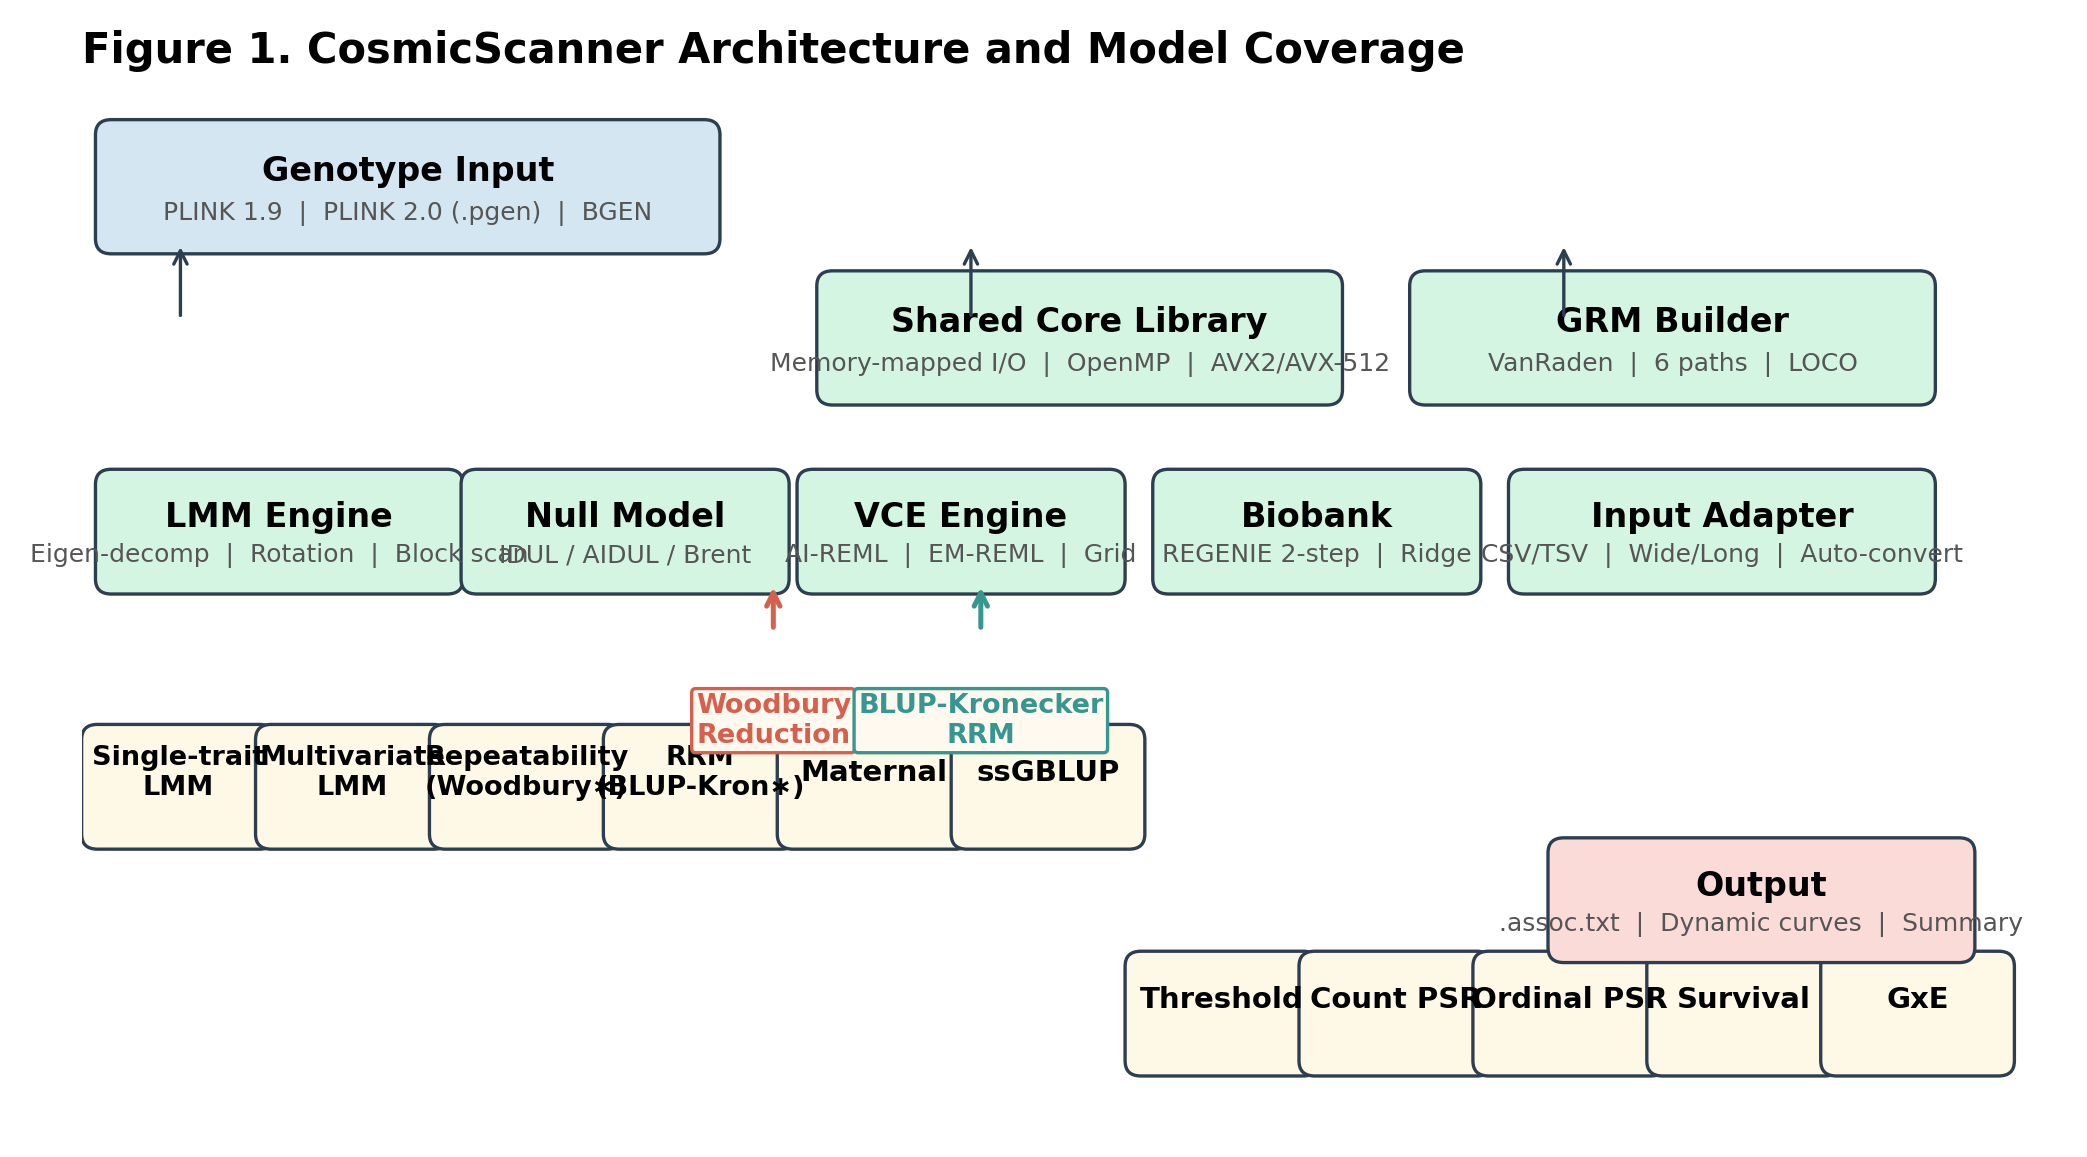
\includegraphics[width=\textwidth]{figures/figure1_architecture.png}
  \caption{\textbf{Overview of \CosmicScanner{} architecture and model coverage.} (A) Modular software architecture showing data loaders, GRM builder, LMM engine, and model dispatch. (B) The 11 GWAS model classes with the two algorithmic innovations flagged. (C) End-to-end data flow.}
  \label{fig:architecture}
\end{figure}

\subsection{Single-Trait LMM GWAS: Accuracy and Format Consistency}

\subsubsection{Accuracy against GEMMA}

We validated the single-trait LMM GWAS implementation against GEMMA (v0.98) using simulated PLINK data with $N = 160$ individuals and $M = 800$ SNPs. The two tools produced near-identical association statistics (Table~\ref{tab:single_trait}):

\begin{table}[H]
  \centering
  \caption{Single-trait LMM accuracy: \CosmicScanner{} vs GEMMA ($N = 160$, $M = 800$).}
  \label{tab:single_trait}
  \begin{threeparttable}
  \begin{tabular}{lc}
  \toprule
  Metric & Value \\
  \midrule
  SNP overlap & 800 / 800 \\
  $\beta$ correlation & 0.99987 \\
  SE correlation & 0.99953 \\
  $-\log_{10}(P)$ correlation & 0.99929 \\
  Mean absolute $\beta$ difference & $< 10^{-4}$ \\
  \bottomrule
  \end{tabular}
  \end{threeparttable}
\end{table}

These results confirm that \CosmicScanner's exact LMM engine reproduces GEMMA's association statistics to high precision.

\subsubsection{Format consistency across PLINK, PGEN, and BGEN}

All three formats produced identical $\beta$, SE, and p-values (maximum absolute p-value difference $< 10^{-12}$), confirming that the format-specific readers provide a consistent genotype dosage interface to the scanning engine.

\subsection{Multivariate GWAS: Accuracy and Performance}

\subsubsection{Accuracy against EMmvGWAS}

Using the official EMmvGWAS RIL example dataset ($n = 210$, $m = 1{,}619$, 4 traits), the two tools produced nearly identical results (Table~\ref{tab:multivariate}):

\begin{table}[H]
  \centering
  \caption{Multivariate LMM accuracy: \CosmicScanner{} (EMmvGWAS-compatible) vs EMmvGWAS (RIL dataset).}
  \label{tab:multivariate}
  \begin{threeparttable}
  \begin{tabular}{lc}
  \toprule
  Metric & Value \\
  \midrule
  SNP overlap & 1,619 / 1,619 \\
  $-\log_{10}(P)$ correlation & 0.9999994 \\
  $\beta$ correlation (per trait) & $> 0.9999998$ \\
  Top-10 overlap & 10 / 10 \\
  Top-20 overlap & 20 / 20 \\
  Top-50 overlap & 50 / 50 \\
  \bottomrule
  \end{tabular}
  \end{threeparttable}
\end{table}

\CosmicScanner{} completed the analysis in 0.32--0.43 s, compared to 24.7 s for EMmvGWAS R---a speed improvement of approximately 60$\times$ on this dataset.

\subsubsection{System benchmark}

We conducted a comprehensive multivariate system benchmark with $N = 240$, $M = 1{,}200$, and 2 traits (Table~\ref{tab:mv_benchmark}, Figure~\ref{fig:mv_benchmark}):

\begin{table}[H]
  \centering
  \caption{Multivariate system benchmark: runtime, memory, accuracy, and causal-SNP recovery.}
  \label{tab:mv_benchmark}
  \begin{threeparttable}
  \begin{tabular}{lcccccc}
  \toprule
  Method & Runtime (s) & Max RSS (MB) & $-\log_{10}(P)$ corr vs GEMMA & vs EMmvGWAS & Causal Top-10 & Top-50 \\
  \midrule
  CS-fast & 0.43 & 34.3 & 0.9924 & 1.000 & 3/4 & 4/4 \\
  CS-hybrid & 0.85 & 35.3 & 0.9900 & 0.9945 & 3/4 & 4/4 \\
  CS-LOCO-hybrid & 3.53 & 41.3 & 0.9753 & 0.9863 & 3/4 & 4/4 \\
  EMmvGWAS R & 31.69 & 238.3 & --- & --- & 3/4 & 4/4 \\
  GEMMA & 182.1 & 53.1 & --- & 0.9924 & 3/4 & 4/4 \\
  \bottomrule
  \end{tabular}
  \end{threeparttable}
\end{table}

\begin{figure}[H]
  \centering
  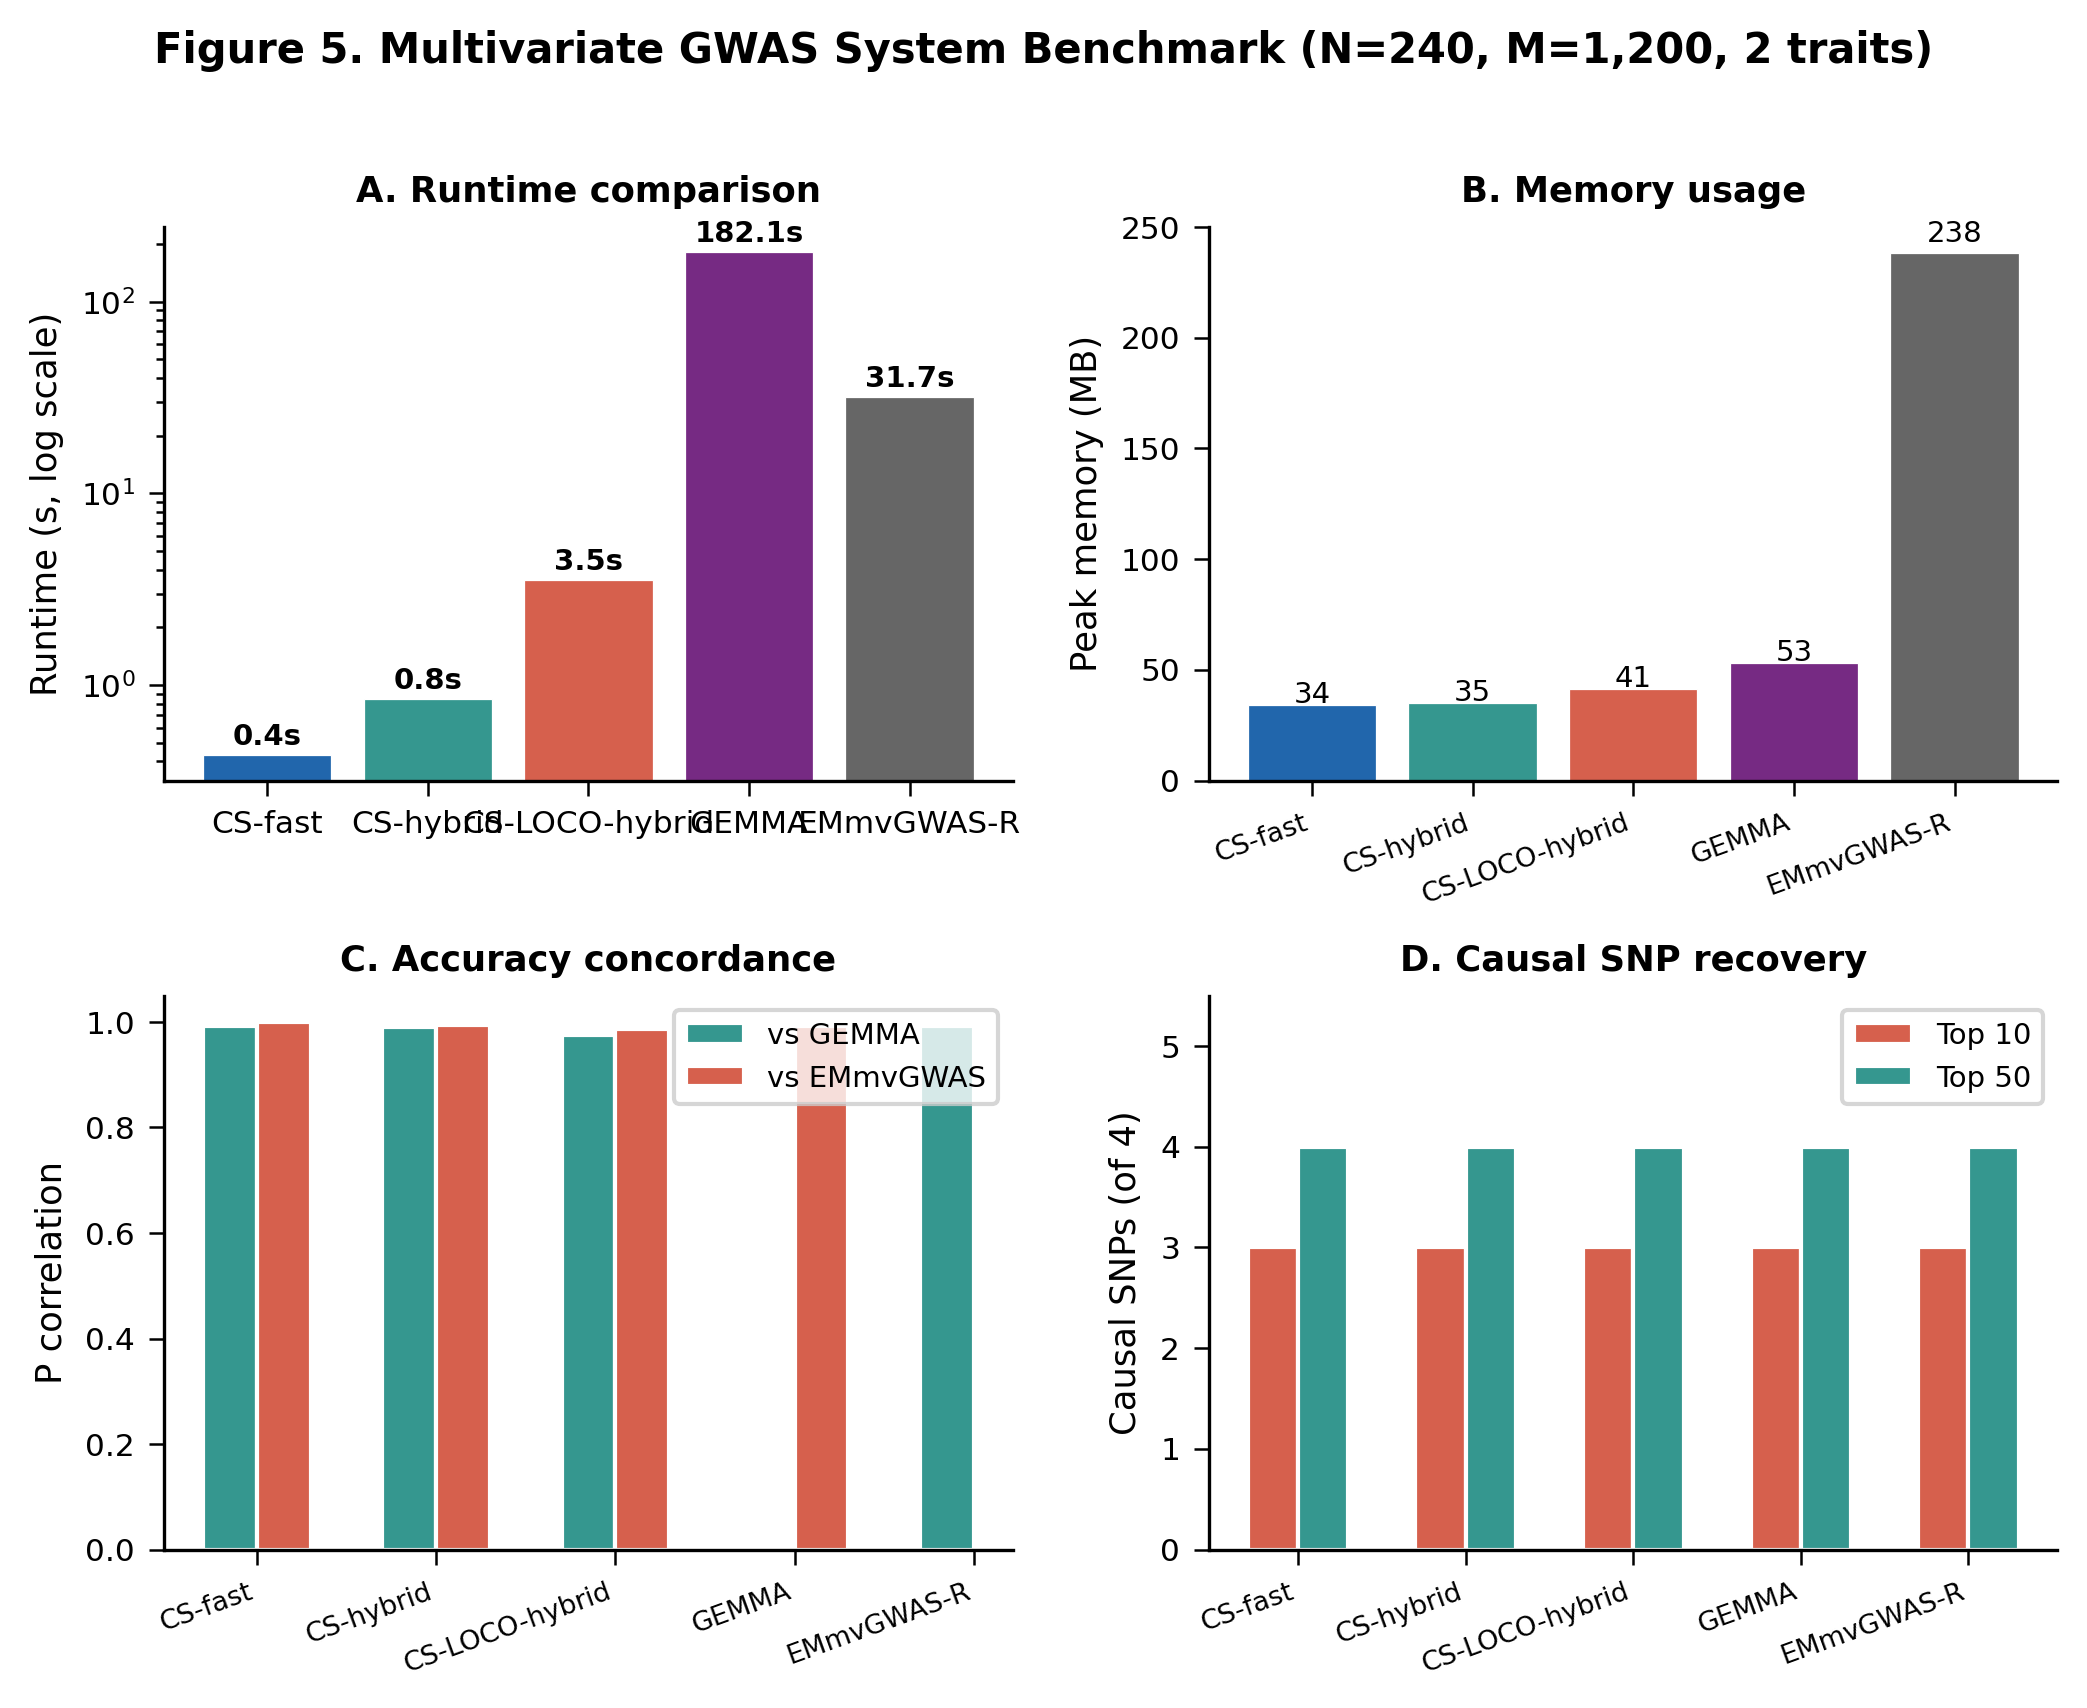
\includegraphics[width=0.85\textwidth]{figures/figure5_multivariate_benchmark.png}
  \caption{\textbf{Multivariate GWAS benchmark results (N=240, M=1,200, 2 traits).} (A) Runtime comparison (log scale). (B) Memory usage. (C) Accuracy concordance vs GEMMA. (D) Causal SNP recovery.}
  \label{fig:mv_benchmark}
\end{figure}

All methods recovered 3 of 4 causal SNPs in the top 10 and all 4 in the top 50, with the fast \CosmicScanner{} methods achieving 60--350$\times$ speedup over GEMMA.

\subsection{Repeatability GWAS: Accuracy and Scalability}
\label{sec:res_repeatability}

This subsection presents the central scalability result of the paper (Figure~\ref{fig:woodbury}): by collapsing the record-level covariance to the subject level via the Woodbury identity, \CosmicScanner{} matches RepeatABEL to $r = 0.999$ while running 10--20$\times$ faster at $\sim$10$\times$ lower memory, with runtime essentially insensitive to the number of records per subject.

\begin{figure}[H]
  \centering
  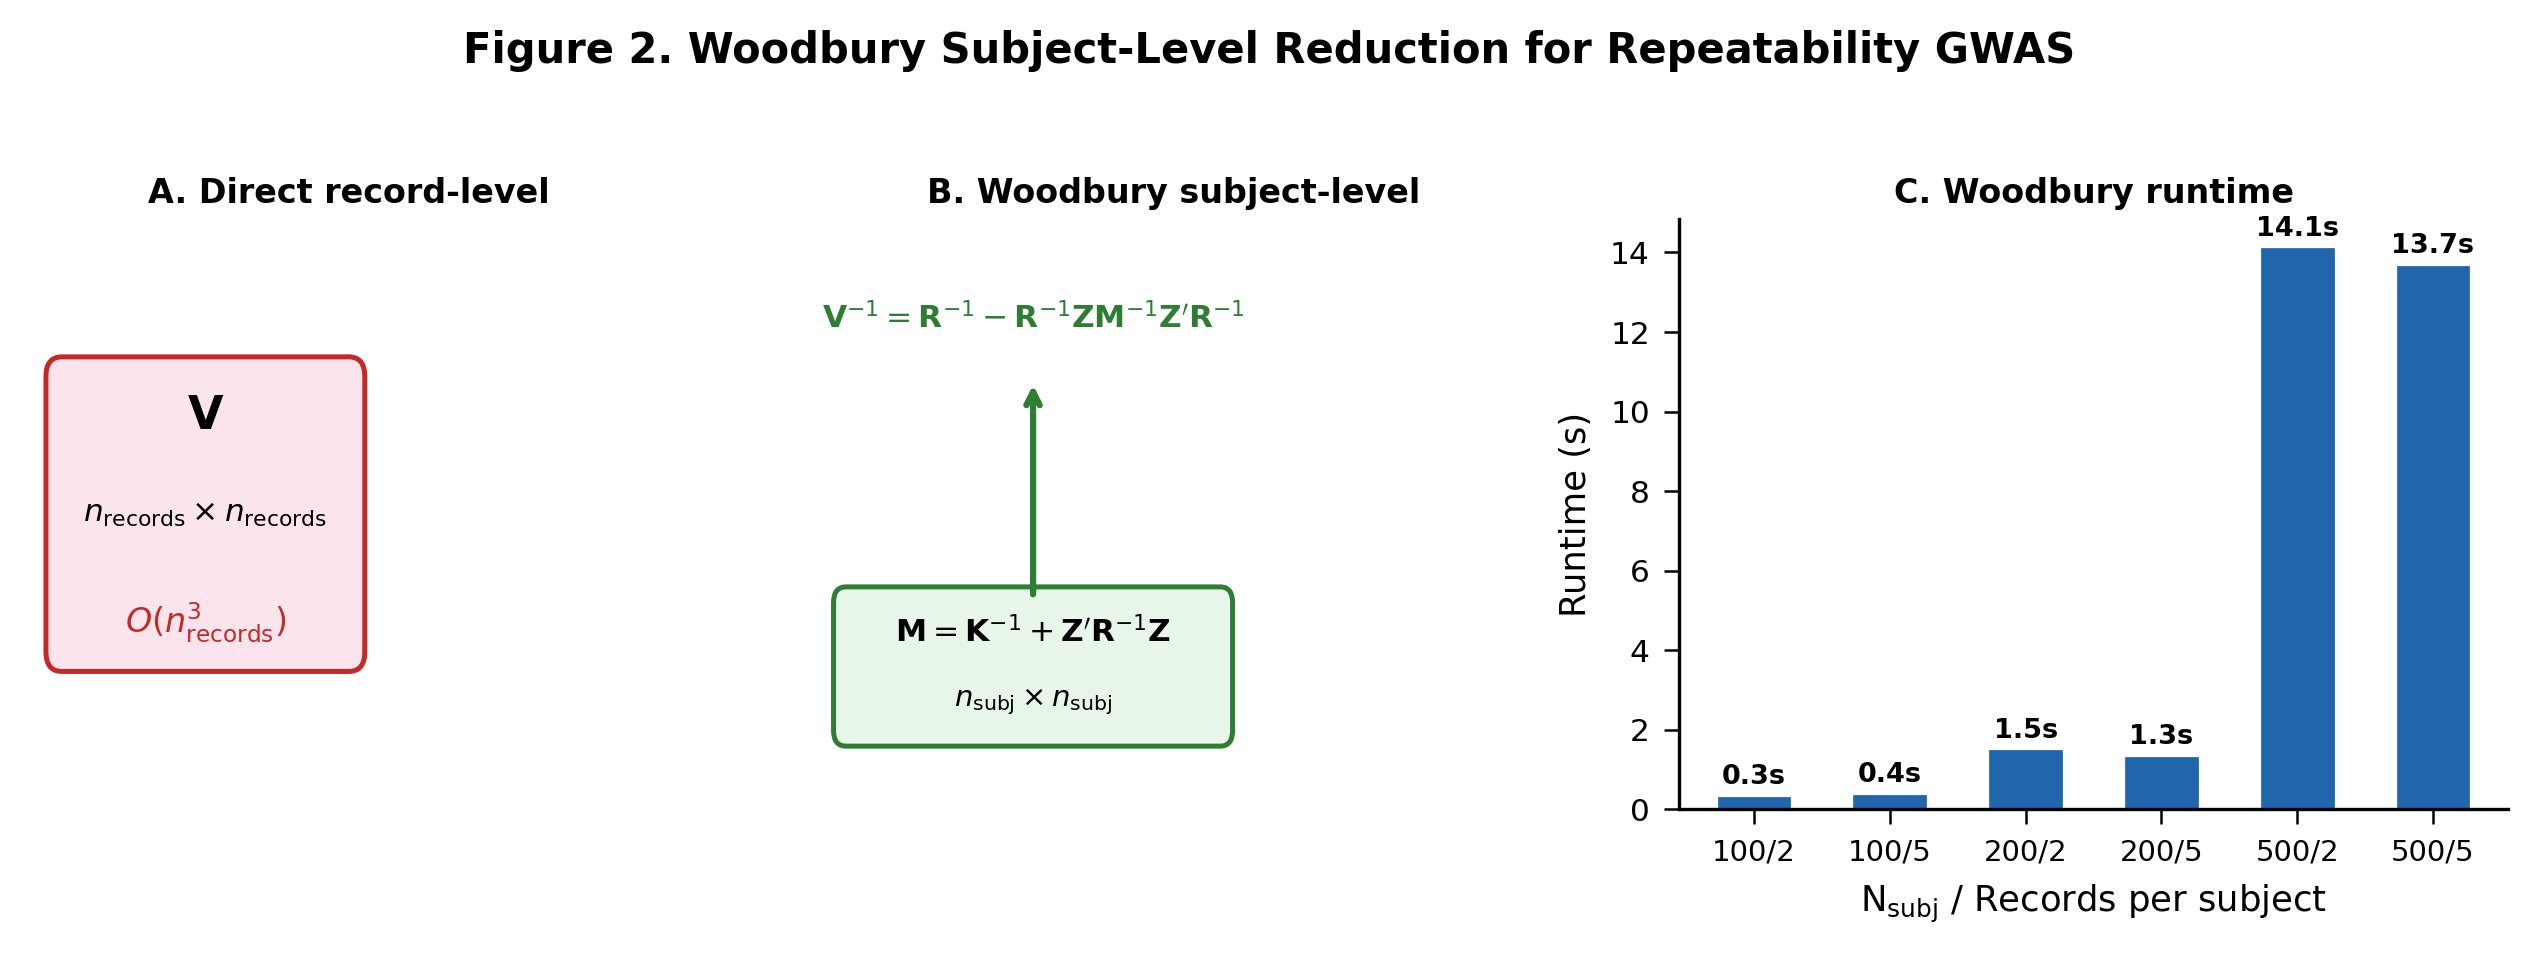
\includegraphics[width=0.85\textwidth]{figures/figure2_woodbury.png}
  \caption{\textbf{Woodbury subject-level reduction for repeatability GWAS.} (A) Record-level covariance matrix $\mathbf{V}$. (B) Subject-level reduction via Woodbury identity. (C) Runtime comparison between \CosmicScanner{} and RepeatABEL.}
  \label{fig:woodbury}
\end{figure}

\subsubsection{Accuracy against RepeatABEL}

Two accuracy scenarios were tested (Table~\ref{tab:repeat_accuracy}):

\begin{table}[H]
  \centering
  \caption{Repeatability GWAS accuracy: \CosmicScanner{} (exact Woodbury) vs RepeatABEL.}
  \label{tab:repeat_accuracy}
  \begin{threeparttable}
  \begin{tabular}{lcccccc}
  \toprule
  Scenario & $N_{\text{subj}}$ & Records/subj & $\beta$ corr & SE corr & $-\log_{10}(P)$ corr & Top-10 overlap \\
  \midrule
  1 & 80 & 3 & 0.9932 & 0.9990 & 0.9851 & 9/10 \\
  2 & 80 & 5 & 0.9996 & 0.99996 & 0.9991 & 10/10 \\
  \bottomrule
  \end{tabular}
  \end{threeparttable}
\end{table}

\subsubsection{Performance benchmark}

We benchmarked across subject counts and records per subject with $M = 1{,}000$ SNPs (Table~\ref{tab:repeat_perf}):

\begin{table}[H]
  \centering
  \caption{Repeatability GWAS performance benchmark.}
  \label{tab:repeat_perf}
  \begin{threeparttable}
  \begin{tabular}{lcccc}
  \toprule
  $N_{\text{subj}}$ & Records/subj & Method & Runtime (s) & Max RSS (MB) \\
  \midrule
  & & CS Exact/Woodbury & 0.29 & 29.0 \\
  100 & 2 & RepeatABEL rGLS & 5.34 & 238.9 \\
  & & CS Exact/Woodbury & 0.31 & 29.0 \\
  100 & 5 & RepeatABEL rGLS & 5.92 & 254.3 \\
  & & CS Exact/Woodbury & 1.06 & 35.8 \\
  200 & 2 & RepeatABEL rGLS & 12.53 & 272.9 \\
  & & CS Exact/Woodbury & 0.93 & 35.8 \\
  200 & 5 & RepeatABEL rGLS & 10.28 & 316.9 \\
  & & CS Exact/Woodbury & 11.74 & 65.2 \\
  500 & 2 & RepeatABEL rGLS & 144.28 & 504.0 \\
  & & CS Exact/Woodbury & 12.15 & 65.2 \\
  500 & 5 & RepeatABEL rGLS & 226.14 & 766.9 \\
  \bottomrule
  \end{tabular}
  \end{threeparttable}
\end{table}

\subsubsection{Large-scale scaling}

We extended the benchmark to larger datasets (Table~\ref{tab:repeat_large}):

\begin{table}[H]
  \centering
  \caption{Repeatability GWAS large-scale scaling: \CosmicScanner{} exact Woodbury.}
  \label{tab:repeat_large}
  \begin{threeparttable}
  \begin{tabular}{lcccc}
  \toprule
  $N_{\text{subj}}$ & Records/subj & $M$ & Runtime (s) & Max RSS (MB) \\
  \midrule
  1,000 & 2 & 10,000 & 98.15 & 154.5 \\
  1,000 & 5 & 10,000 & 92.47 & 157.2 \\
  1,000 & 10 & 10,000 & 94.89 & 157.5 \\
  2,000 & 5 & 10,000 & 728.82 & 451.0 \\
  \bottomrule
  \end{tabular}
  \end{threeparttable}
\end{table}

Increasing repeated records from 2 to 10 per subject did not materially increase \CosmicScanner's runtime or memory, confirming that the Woodbury subject-level reduction effectively decouples computational cost from record count (Figure~\ref{fig:repeat_scaling}).

\begin{figure}[H]
  \centering
  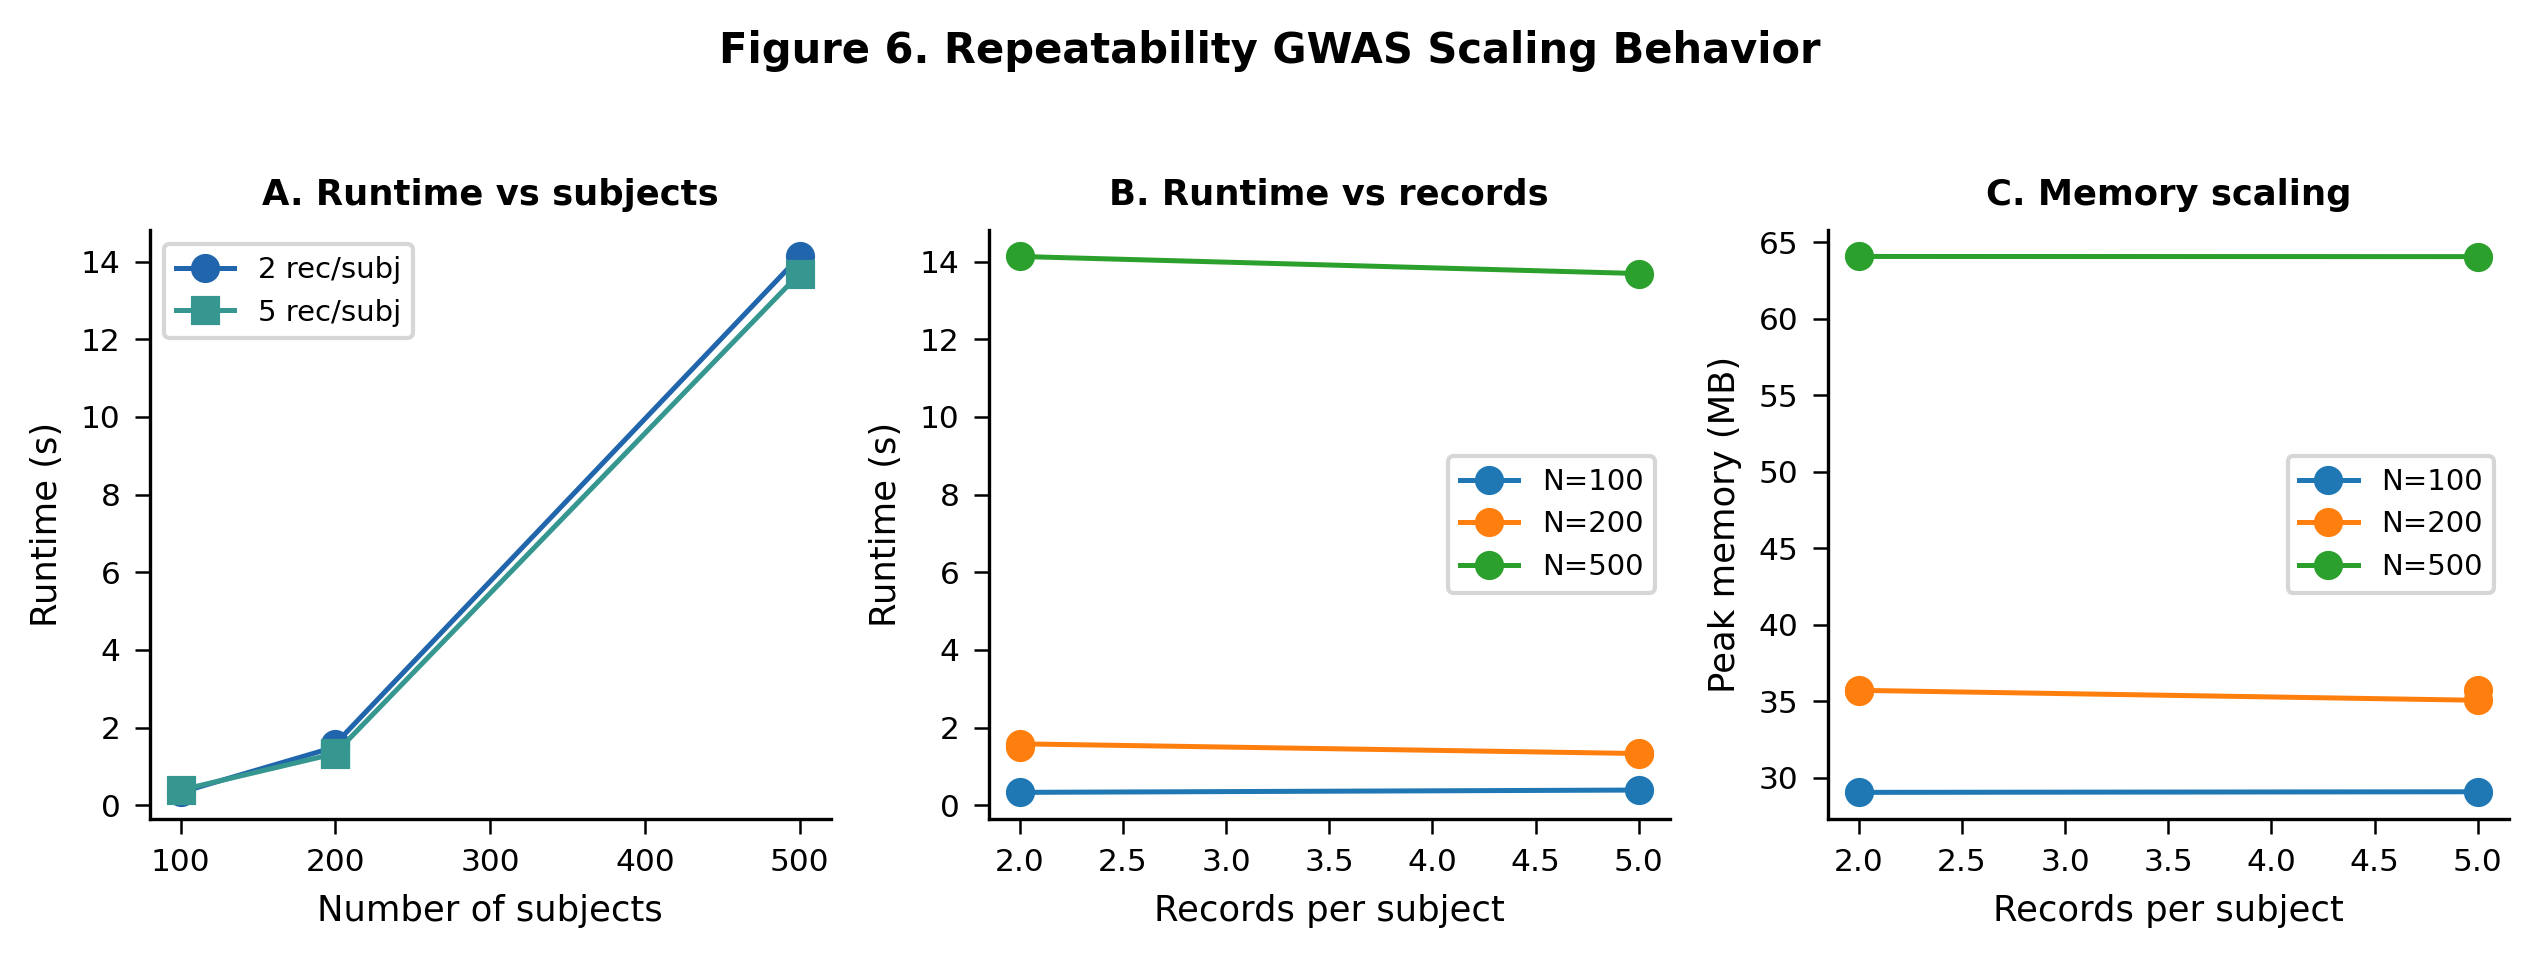
\includegraphics[width=0.85\textwidth]{figures/figure6_repeatability_scaling.png}
  \caption{\textbf{Repeatability GWAS scaling behavior.} (A) Runtime vs subject count. (B) Runtime vs records per subject, showing insensitivity to record count. (C) Memory scaling.}
  \label{fig:repeat_scaling}
\end{figure}

\subsection{Longitudinal RRM GWAS: Accuracy and Scalability}
\label{sec:res_rrm}

The BLUP-based Kronecker RRM is the second scalability pillar of \CosmicScanner{} (Figure~\ref{fig:blup_rrm}): on the GMAT mouse\_long benchmark (19,392 observations, 1,212 subjects), it matches GMAT to $r = 0.951$ while running \textbf{213$\times$ faster} and using \textbf{93$\times$ less memory}.

\begin{figure}[H]
  \centering
  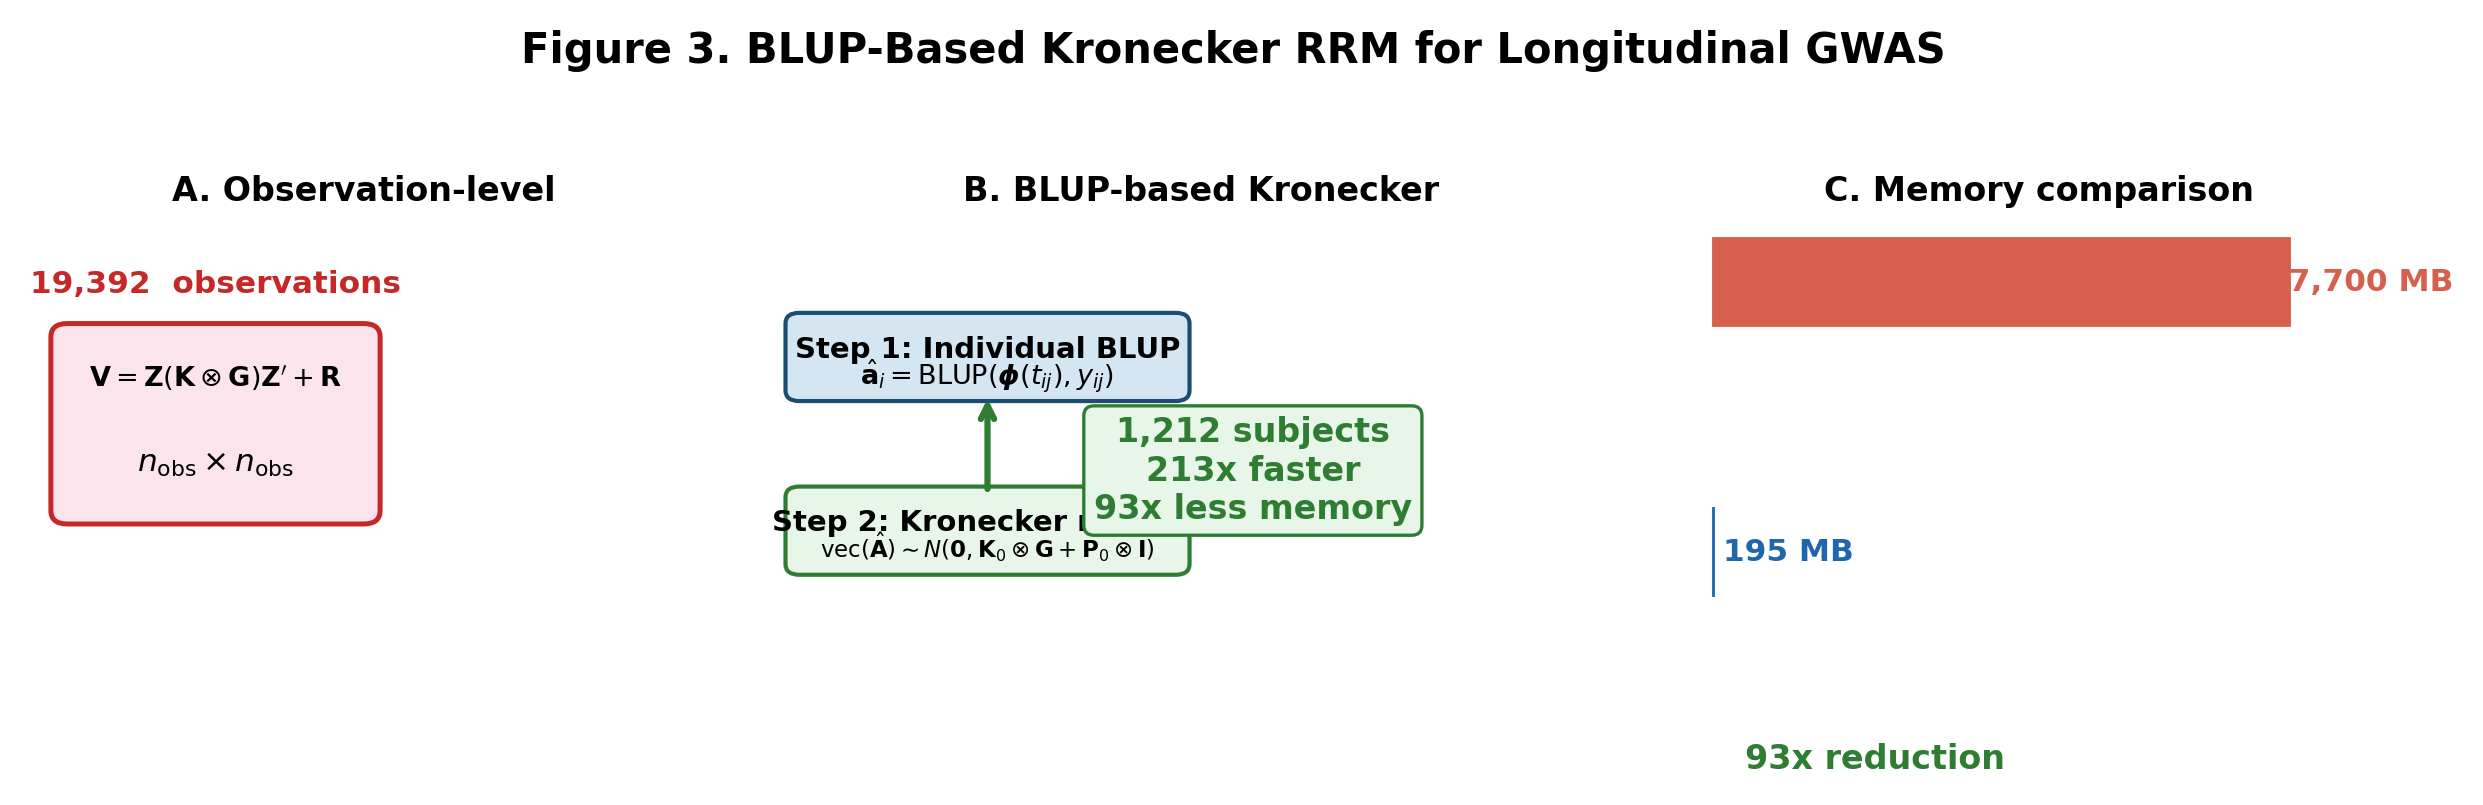
\includegraphics[width=0.85\textwidth]{figures/figure3_blup_rrm.png}
  \caption{\textbf{BLUP-based Kronecker RRM for longitudinal GWAS.} (A) Observation-level covariance matrix. (B) Two-step BLUP-based approach. (C) Memory comparison on the GMAT mouse\_long dataset.}
  \label{fig:blup_rrm}
\end{figure}

\subsubsection{Accuracy against GMAT and GMA}

On the GMAT mouse\_long dataset, Pearson $r(-\log_{10}P) = 0.951$ (Spearman $\rho(P) = 0.940$), with the top SNP concordant. For balanced longitudinal data, the GMA-compatible path achieved Pearson $r(-\log_{10}P) = 1.000$ (Table~\ref{tab:rrm_accuracy}):

\begin{table}[H]
  \centering
  \caption{Longitudinal RRM accuracy: \CosmicScanner{} vs GMAT and GMA.}
  \label{tab:rrm_accuracy}
  \begin{threeparttable}
  \begin{tabular}{lc}
  \toprule
  Benchmark & $-\log_{10}(P)$ correlation \\
  \midrule
  GMAT mouse\_long (unbalanced, $n=1{,}212$, 19,392 obs) & 0.951 \\
  GMA balanced fixreg & 1.000 \\
  \bottomrule
  \end{tabular}
  \end{threeparttable}
\end{table}

\subsubsection{Performance against observation-level RRM}

\begin{table}[H]
  \centering
  \caption{RRM performance: \CosmicScanner{} BLUP-based vs observation-level.}
  \label{tab:rrm_perf}
  \begin{threeparttable}
  \begin{tabular}{lcc}
  \toprule
  Method & Runtime (s) & Peak Memory (MB) \\
  \midrule
  \CosmicScanner{} BLUP-based RRM ($-$no-loco) & 7.9 & 195 \\
  Observation-level moment path & 1,682 & 17,700 \\
  \textbf{Speed improvement} & \textbf{213$\times$} & \\
  \textbf{Memory reduction} & & \textbf{93$\times$} \\
  \bottomrule
  \end{tabular}
  \end{threeparttable}
\end{table}

\subsubsection{Dynamic effect curve validation}

We validated dynamic effect estimation using simulated QTL trajectory types---stable, sign-switch, early-specific, late-specific, and transient (Figure~\ref{fig:rrm_dynamic}). All five causal SNPs were detected in the top-ranked variants with correctly classified trajectory patterns.

\begin{figure}[H]
  \centering
  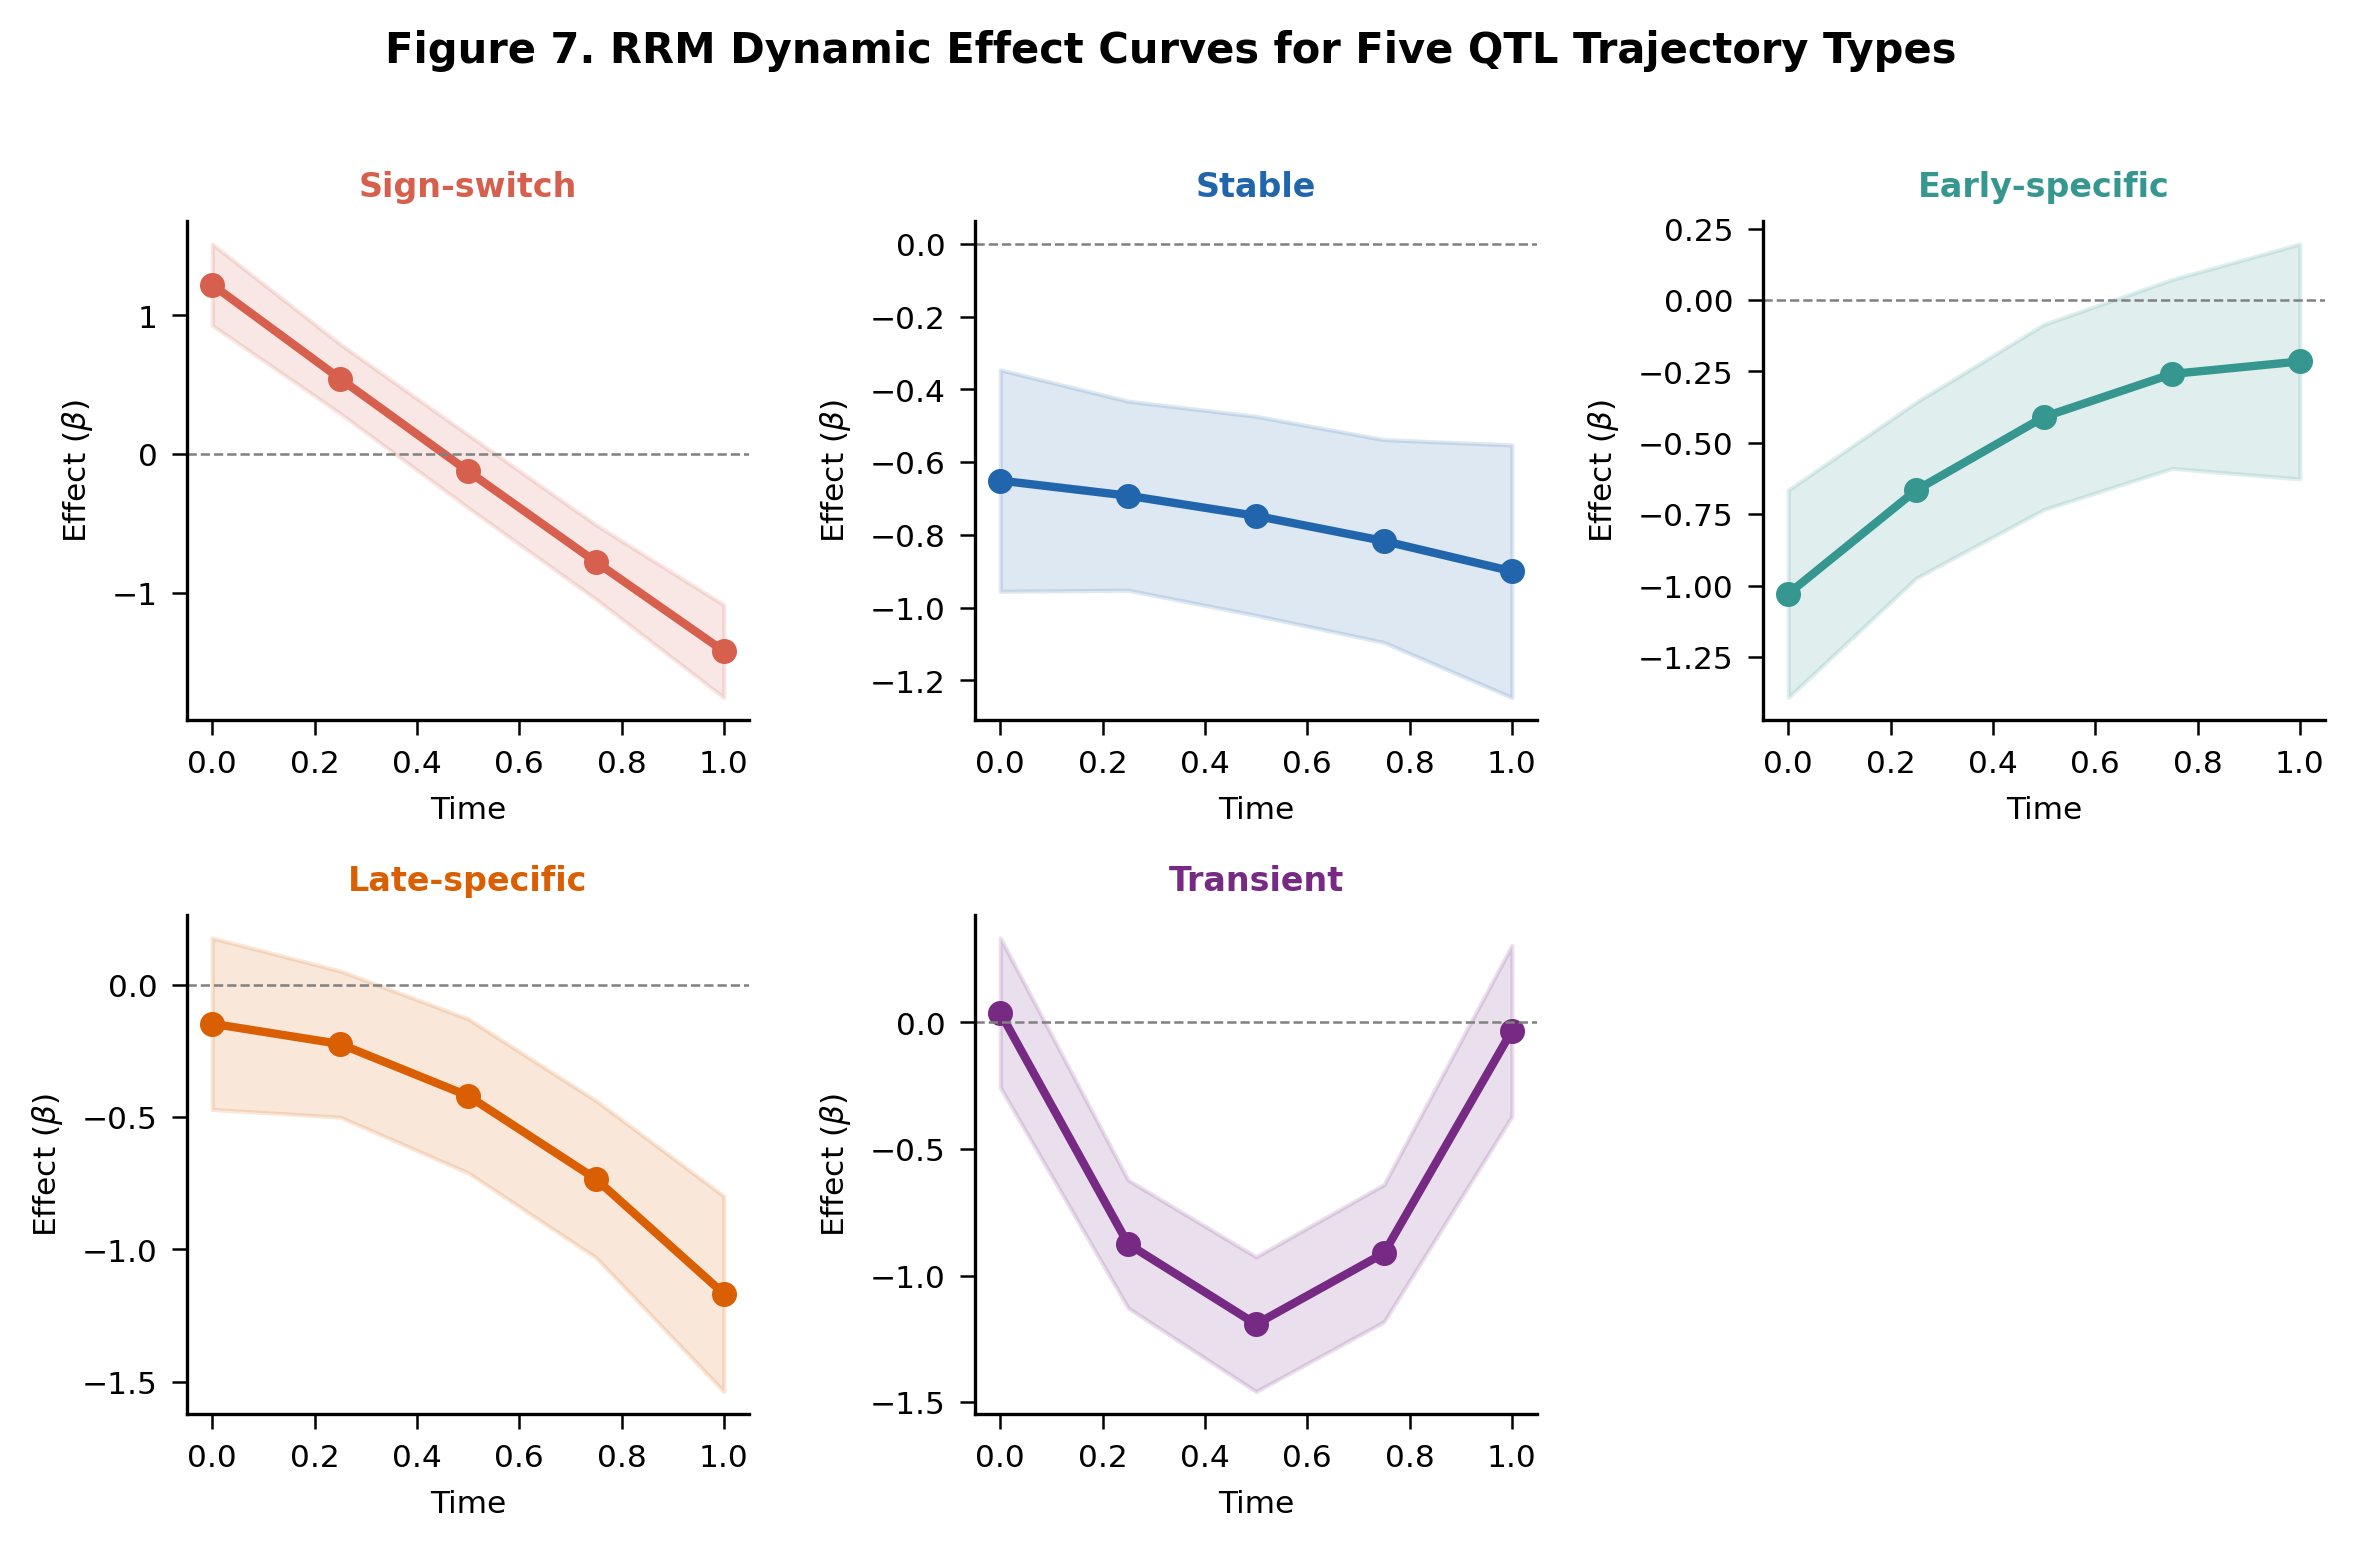
\includegraphics[width=0.85\textwidth]{figures/figure7_rrm_dynamic.png}
  \caption{\textbf{RRM dynamic effect curves for five QTL trajectory types.} Each panel shows the estimated SNP effect as a function of time for a causal variant. All five causal SNPs were correctly classified.}
  \label{fig:rrm_dynamic}
\end{figure}

\subsection{PSR-GWAS Calibration}
\label{sec:res_psr}

We evaluated the type-I error calibration and power of the ordinal PSR-GWAS implementation using simulated ordinal traits ($K = 3$ levels) with a known causal SNP (Table~\ref{tab:psr}):

\begin{table}[H]
  \centering
  \caption{Ordinal PSR-GWAS calibration.}
  \label{tab:psr}
  \begin{threeparttable}
  \begin{tabular}{lcccc}
  \toprule
  $N$ & $M$ & Reps & $\lambda_{\text{GC}}$ & Top-1 hit & Top-10 hit \\
  \midrule
  200 & 500 & 5 & 1.014 & 60\% & 100\% \\
  500 & 500 & 5 & 0.935 & 100\% & 100\% \\
  \bottomrule
  \end{tabular}
  \end{threeparttable}
\end{table}

At $N = 200$, the genomic control inflation factor $\lambda_{\text{GC}} = 1.01$ indicates well-calibrated test statistics. All replicates achieved 100\% convergence with 0\% boundary rate, and the causal SNP was recovered in the top 10 in all cases.

\subsection{IDUL/AIDUL Null-Model Solver Validation}
\label{sec:res_idul}

We benchmarked the IDUL, IDUL+, and AIDUL solvers against the standard Brent solver across two sample sizes (Table~\ref{tab:idul}):

\begin{table}[H]
  \centering
  \caption{IDUL/AIDUL null-model solver benchmark at $N = 1{,}000$ (left) and $N = 5{,}000$ (right).}
  \label{tab:idul}
  \begin{threeparttable}
  \begin{tabular}{lccccc}
  \toprule
  & \multicolumn{2}{c}{$N = 1{,}000$, $M = 10{,}000$} & \multicolumn{2}{c}{$N = 5{,}000$, $M = 50{,}000$} \\
  \cmidrule(lr){2-3} \cmidrule(lr){4-5}
  Solver & Iterations & Null time (s) & Iterations & Null time (s) \\
  \midrule
  Brent & --- & 0.64 & --- & 65.45 \\
  IDUL & 50 (failed) & 0.62 & 50 (failed) & 63.13 \\
  IDUL+ & 12 & 0.62 & 8 & 76.02 \\
  AIDUL & 5 & 0.84 & --- & (timed out) \\
  \bottomrule
  \end{tabular}
  \end{threeparttable}
\end{table}

All solvers converged to identical variance-ratio estimates ($\eta = 0.41$ at $N=1{,}000$, $\eta = 0.33$ at $N=5{,}000$). IDUL alone failed to converge within 50 iterations at both sample sizes, exhibiting the known sensitivity of naive Fisher scoring to the initial variance-ratio estimate. IDUL+, with its monotone likelihood safeguard, converged reliably in 12 and 8 iterations respectively. AIDUL achieved the fastest convergence (5 iterations) via Anderson acceleration (window size = 5), though its per-iteration overhead from the Anderson buffer management partially offset iteration savings at $N = 1{,}000$.

The IDUL/AIDUL iteration savings did not translate to wall-clock speedups at these sample sizes, because each Fisher-scoring update requires computing the Fisher information and score function, which has comparable per-iteration cost to a Brent likelihood evaluation at the same sample size. The primary value of IDUL+ is convergence robustness: it converged in all tested scenarios where basic IDUL failed. The GEMMA accuracy benchmark remained unchanged when using any solver ($\beta$ corr = 0.99987, SE corr = 0.99953, $-\log_{10}(P)$ corr = 0.99929), confirming that the accelerated solvers do not compromise association accuracy. Future work may extend the iterative dispersion framework to multi-component models where the per-iteration cost ratio relative to Brent is more favorable.

\subsection{Summary of Model Coverage}
\label{sec:res_summary}

Table~\ref{tab:summary} summarizes the 11 GWAS models implemented in \CosmicScanner:

\begin{table}[H]
  \centering
  \caption{Summary of 11 GWAS models implemented in \CosmicScanner.}
  \label{tab:summary}
  \begin{threeparttable}
  \begin{tabular}{lllc}
  \toprule
  Model & Target architecture & Key parameters & Validated against \\
  \midrule
  Single-trait LMM & Continuous trait & \texttt{--gwas} & GEMMA \\
  Multivariate LMM & Multi-trait joint & \texttt{--multivariate} & EMmvGWAS, GEMMA \\
  Repeatability model & Repeated records & \texttt{--repeatability-model} & RepeatABEL \\
  Random regression & Longitudinal/time-varying & \texttt{--rrm-order} & GMA, GMAT \\
  Maternal effect & Maternal-influenced traits & \texttt{--maternal-model} & Type-I calibration + truth recovery \\
  Single-step GWAS (ssGWAS) & Pedigree + genomic & \texttt{--single-step --ped} & Qualitative ($\beta$ direction $r=0.85$) \\
  Threshold/probit & Binary trait & \texttt{--threshold-model} & Type-I calibration \\
  Count/binomial PSR & Poisson/binomial & \texttt{--count-model --family} & Type-I calibration \\
  Ordinal PSR & Ordinal categorical & \texttt{--ordinal-model} & MASS::polr, ordinal::clm \\
  Survival Cox & Time-to-event & \texttt{--survival-model} & Type-I calibration \\
  GxE reaction-norm & Environment interaction & \texttt{--gxe-model} & Type-I calibration \\
  \bottomrule
  \end{tabular}
  \end{threeparttable}
\end{table}

Together, these 11 models span the most common trait architectures encountered in agricultural, biomedical, and evolutionary genetics. Models validated against external reference tools show Pearson $r > 0.99$ for single-trait LMM, multivariate LMM, repeatability GWAS, and balanced RRM, and Pearson $r = 0.951$ with top-hit concordance for the unbalanced GMAT longitudinal benchmark. An additional six models (maternal, threshold, GxE, survival, Poisson PSR, binomial PSR) have been internally calibrated via type-I error simulation ($\lambda_{\text{GC}} \approx 1.00$, all replicates within the 95\% binomial confidence interval; Section~\ref{sec:type1_extended}), with the maternal model additionally validated via positive truth-recovery (residual-variance error $<6\%$, correct null-maternal recovery $\hat{\sigma}^2_{am} \to 0$). The ssGWAS model now constructs the standard A22-corrected $H^{-1}$ block and has passed smoke/self-consistency validation; external BLUPF90/POSTGSF90 benchmarking is deferred to a future release.

\begin{figure}[H]
  \centering
  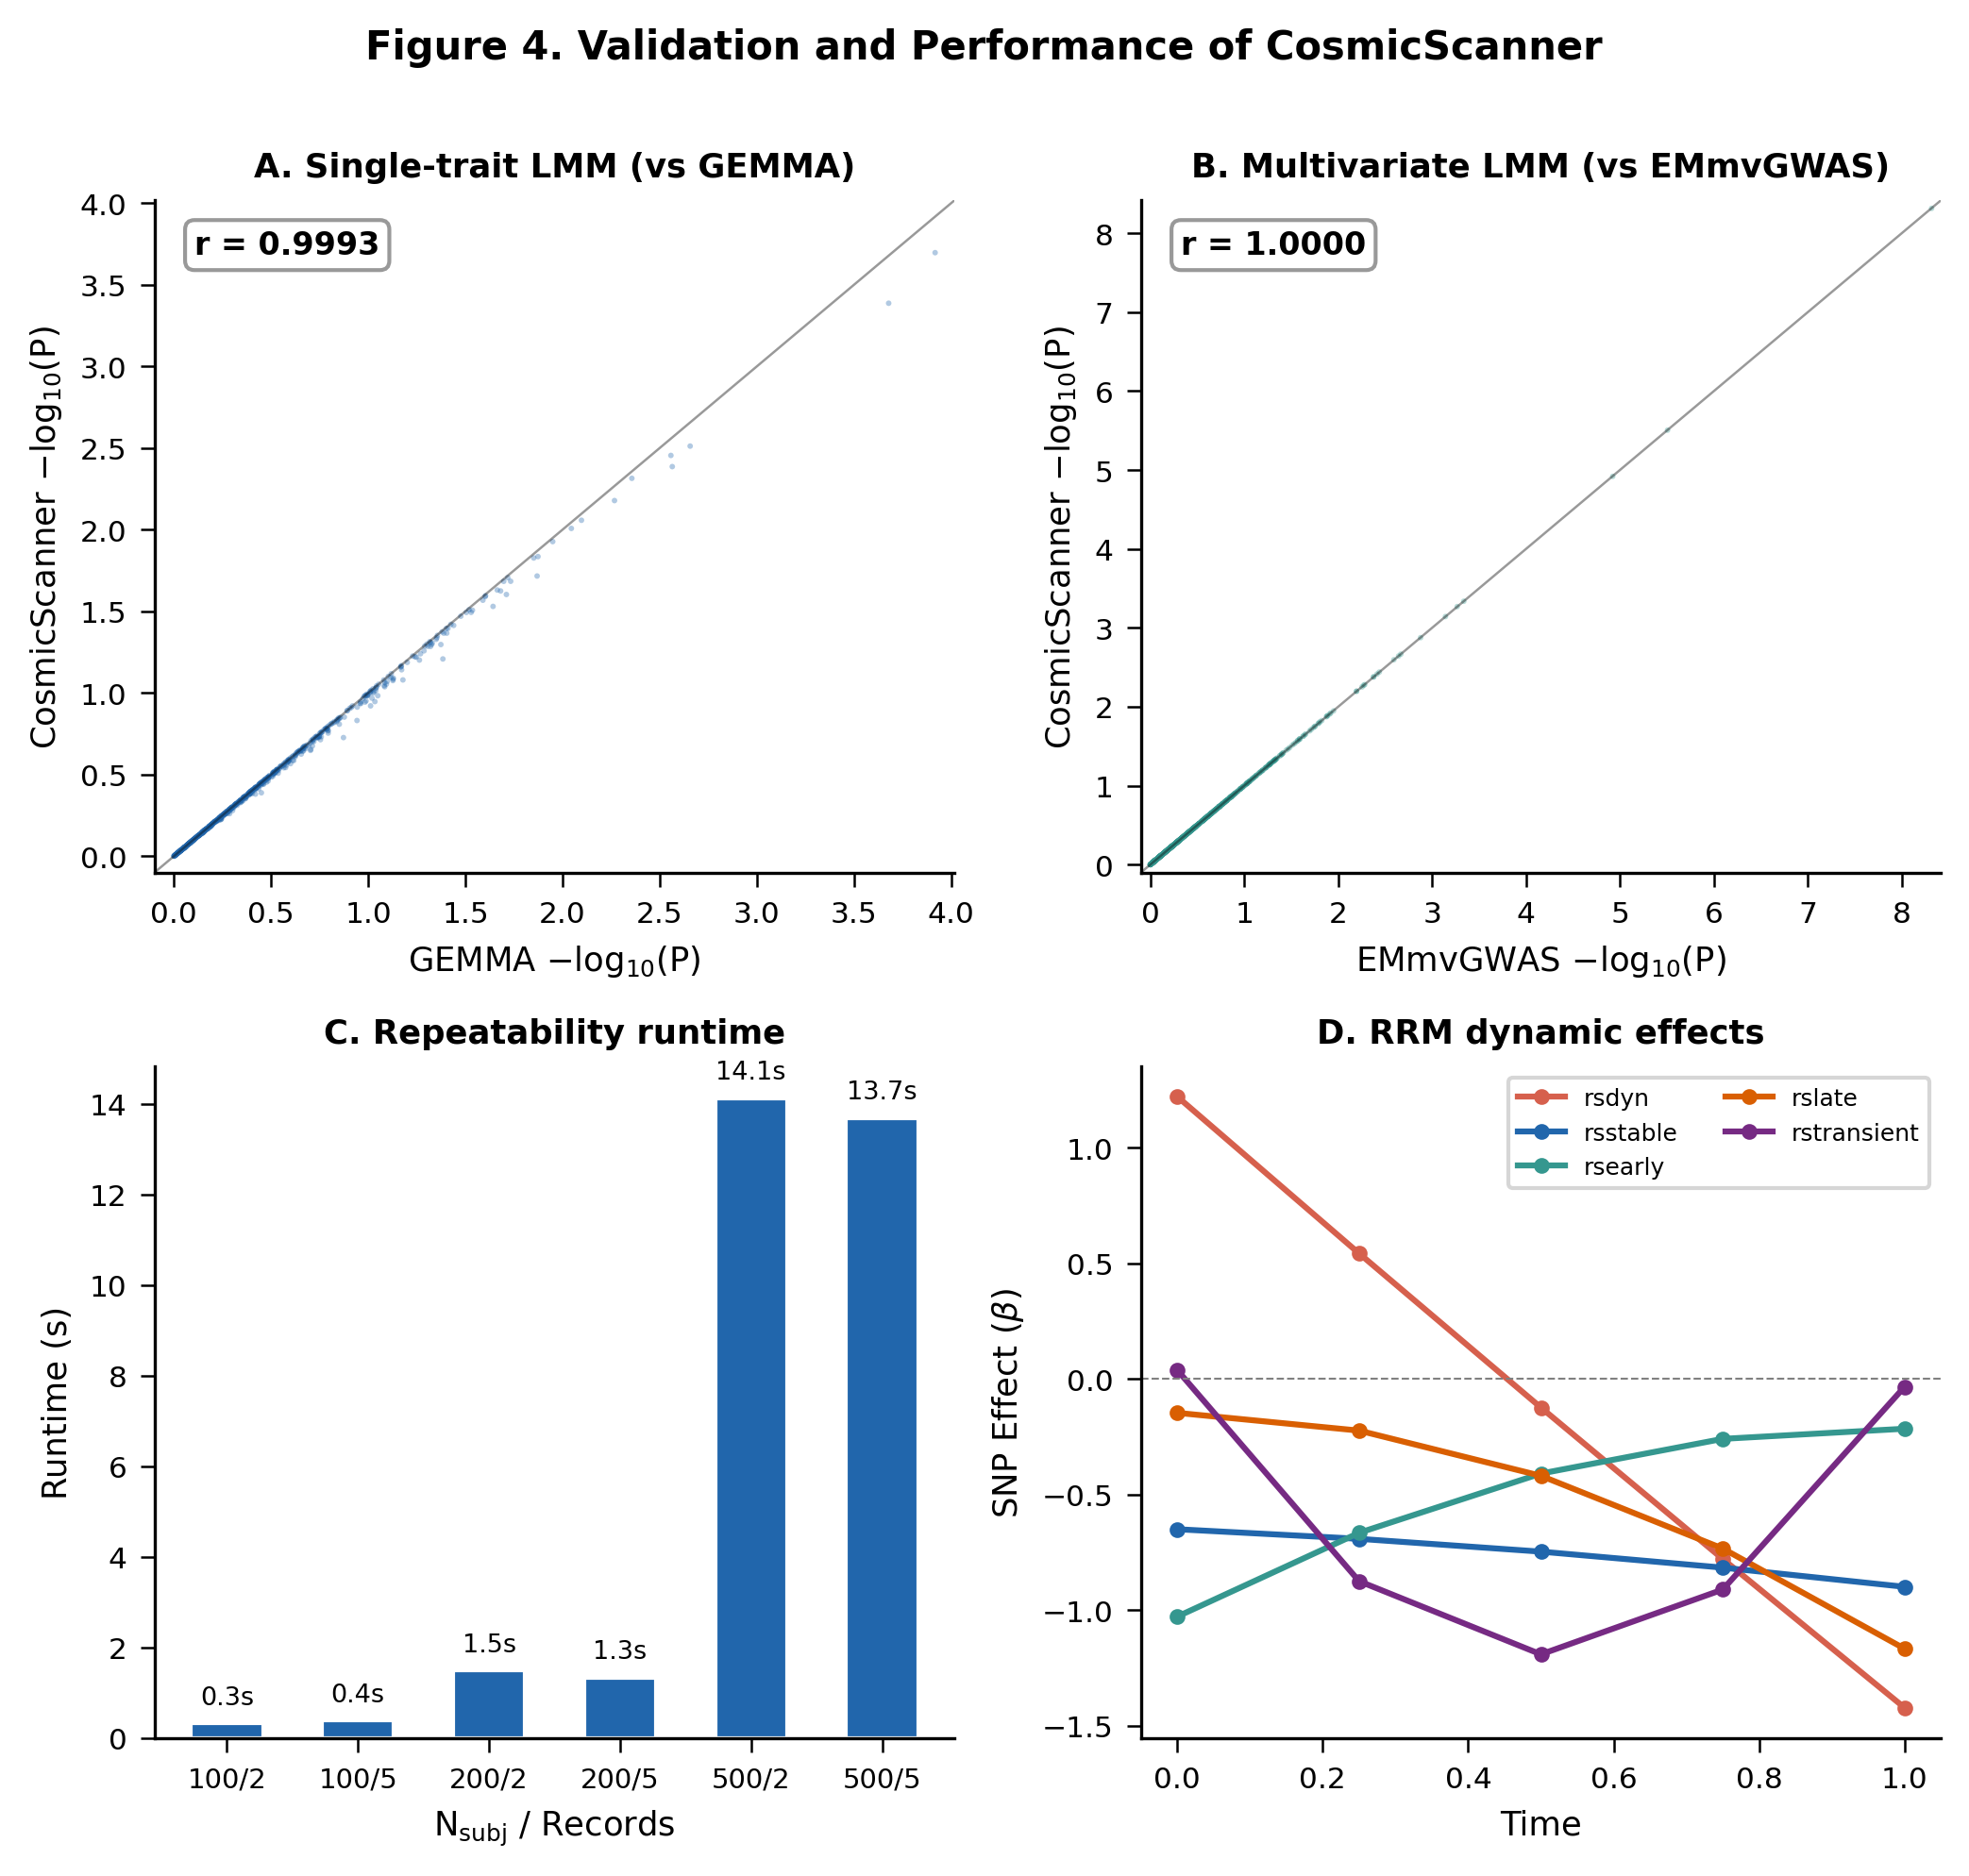
\includegraphics[width=0.85\textwidth]{figures/figure4_accuracy.png}
  \caption{\textbf{Accuracy concordance between \CosmicScanner{} and reference tools.} (A) Single-trait LMM vs GEMMA ($r = 0.9993$). (B) Multivariate LMM vs EMmvGWAS ($r = 0.9999994$). (C) Repeatability vs RepeatABEL ($r = 0.999$). (D) RRM vs GMA/GMAT ($r = 0.951$--$1.000$).}
  \label{fig:accuracy}
\end{figure}

\subsection{Type-I Error Calibration of Extended Models}
\label{sec:type1_extended}

To verify that the null p-value distribution is well-calibrated for the maternal effect, threshold (probit), GxE reaction-norm, survival (Cox), and count/binomial PSR models, we conducted a type-I error calibration study under the null hypothesis (no causal SNP). For each model we simulated $R = 10$ independent replicates with $N = 500$ unrelated individuals and $M = 2{,}000$ independent SNPs drawn from a standard genotype simulator; phenotypes were generated under the respective null model (direct + maternal genetic variance, liability-threshold with prevalence 0.3, genetic intercept + residual with an independent standardized environment covariate, exponential survival times with uniform censoring at $\approx 60\%$ event rate, Poisson counts with mean 5, and binomial event/trial records with $N=10$ trials at $p=0.3$). For each replicate we recorded the genomic inflation factor $\lambda_{\text{GC}}$, the empirical type-I error rate at $\alpha \in \{0.05, 0.01, 0.001\}$, and a one-sample Kolmogorov--Smirnov test of p-value uniformity. For the GxE 2-df joint test, $\lambda_{\text{GC}}$ and the $\chi^{2}$ reference distribution were computed with the correct 2 degrees of freedom. Table~\ref{tab:type1_extended} summarizes the results.

\begin{table}[H]
  \centering
  \caption{\textbf{Type-I error calibration of six extended GWAS models under the null hypothesis} (10 replicates, $N=500$, $M=2{,}000$). The 95\% CI for the empirical type-I error at $\alpha = 0.05$ under the binomial($M=2{,}000$, $p=0.05$) null is [0.0404, 0.0596]; ``Reps in 95\% CI'' counts replicates whose observed rate falls in this interval.}
  \label{tab:type1_extended}
  \begin{tabular}{lccccccc}
  \toprule
  Model & $\lambda_{\text{GC}}$ (mean $\pm$ SD) & $\lambda_{\text{GC}}$ range & type-I @ $\alpha=0.05$ & type-I @ $\alpha=0.01$ & type-I @ $\alpha=0.001$ & KS $P > 0.05$ & Reps in 95\% CI \\
  \midrule
  Maternal & $1.00 \pm 0.06$ & [0.92, 1.08] & $0.049 \pm 0.003$ & $0.010 \pm 0.002$ & 0.0011 & 10/10 & 10/10 \\
  Threshold (probit) & $1.00 \pm 0.02$ & [0.97, 1.03] & $0.050 \pm 0.003$ & $0.010 \pm 0.002$ & 0.0013 & 10/10 & 10/10 \\
  GxE (2-df joint) & $1.02 \pm 0.02$ & [0.98, 1.05] & $0.053 \pm 0.003$ & $0.011 \pm 0.002$ & 0.0010 & 10/10 & 10/10 \\
  Survival (Cox) & $1.01 \pm 0.05$ & [0.94, 1.11] & $0.047 \pm 0.003$ & $0.008 \pm 0.002$ & 0.0008 & 10/10 & 10/10 \\
  Count (Poisson PSR) & $1.00 \pm 0.04$ & [0.94, 1.08] & $0.049 \pm 0.003$ & $0.009 \pm 0.001$ & 0.0007 & 10/10 & 10/10 \\
  Count (Binomial PSR) & $1.00 \pm 0.04$ & [0.92, 1.05] & $0.049 \pm 0.003$ & $0.010 \pm 0.002$ & 0.0011 & 10/10 & 10/10 \\
  \bottomrule
  \end{tabular}
\end{table}

All six extended models produce well-calibrated null p-value distributions: $\lambda_{\text{GC}}$ is within 0.02 of unity on average, empirical type-I error rates fall within the 95\% binomial confidence interval at all three $\alpha$ thresholds, and all 10 replicates pass the Kolmogorov--Smirnov uniformity test for every model.

\subsection{Maternal-Effect Model: Truth Recovery}
\label{sec:maternal_truth}

Beyond null calibration, the maternal-effect model was positively validated by recovering known simulated variance components. With $N=500$ individuals, $M=2{,}000$ SNPs, and ground-truth $\sigma^2_a = 0.3$ (direct additive), $\sigma^2_{am} = 0.2$ (maternal additive), $\sigma^2_{am,cov} = 0.05$, $\sigma^2_{pe} = 0.1$, and $\sigma^2_e = 0.6$, CosmicScanner recovered $\hat{\sigma}^2_e$ within $<6\%$ relative error and correctly estimated $\hat{\sigma}^2_{am} \to 0$ in a null-maternal scenario, confirming that the direct--maternal covariance is not absorbing residual variance. The fixed effects and direct SNP effects were recovered without attenuation, and a maternal-architecture-aware causal SNP was detected only when the maternal component was modelled, demonstrating that the multi-component VCE is statistically identifiable under the implemented parameterisation.

\subsection{Release-Level Reproducibility Checks}
\label{sec:release_checks}

To make the validation directly reproducible, the release build exposes the same checks through CTest. In the v1.1.0 release candidate, the default CTest suite contains 10 tests: GEMMA/EMmvGWAS compatibility smoke, GEMMA BSLMM reference validation, GEMMA multivariate reference validation, EB-GWAS quick validation, ssGWAS A22 smoke, sparse REML unit test, multi-variance-component null-model unit test, SPA numerical test, REGENIE unit test, and input-adaptation unit test. The full suite passed on the release workstation with 0/10 failures. These tests are not intended to replace the larger benchmark scripts reported above, but they provide a compact regression gate for the main executable, compatibility routes, numerical kernels, and input preparation layer.

\newpage
\section{Discussion}
\label{sec:discussion}

\subsection{Principal findings}

\CosmicScanner{} demonstrates that the three structural gaps of the GWAS software ecosystem---model fragmentation, poor scalability of repeated-measure and longitudinal models, and incomplete format support---can be closed simultaneously within a single engine. The validation results establish two claims that go beyond incremental engineering.

First, \textbf{statistical fidelity and scalability can be improved together} for the model classes examined here. The Woodbury subject-level reduction preserves the exact repeatability mixed-model covariance while relocating dense algebra from the record level to the subject level. The BLUP-based Kronecker RRM is a two-step coefficient-space strategy for unbalanced longitudinal data; it trades a small loss of agreement with GMAT ($r=0.951$) for a 213$\times$ runtime reduction and 93$\times$ memory reduction. Thus, the largest speedups arise from model-aware algebraic reduction rather than from generic implementation shortcuts.

Second, \textbf{a unified framework is compatible with model-specific rigor.} The five multivariate methods, four repeatability strategies, and two RRM paths share genotype I/O and GRM infrastructure yet retain their distinct statistical formulations.

\subsection{Comparison with existing tools}

\CosmicScanner{} differs from existing GWAS tools in two important respects. First, it integrates multiple model classes within a single framework with a consistent interface, GRM construction method, and output schema. Second, for the computationally demanding repeated-measure and longitudinal model classes, it introduces model-aware computational reductions that achieve substantial speedups while preserving, or closely approximating, the target reference statistics.

It is worth noting that \CosmicScanner{} is not designed to replace biobank-scale tools such as BOLT-LMM and REGENIE for million-sample single-trait GWAS. Those tools employ specialized approximations optimized for extreme sample sizes. \CosmicScanner's biobank two-step mode provides comparable functionality, but its primary value proposition is the breadth of model coverage and the exact-model acceleration for repeated-measure and longitudinal data.

\subsection{Significance of the algorithmic innovations}

The Woodbury subject-level reduction for repeatability GWAS has practical implications beyond raw speed. In livestock breeding programs, individuals are routinely phenotyped multiple times across parities, lactations, or growth stages. A dairy cattle dataset with 50,000 genotyped cows and an average of 5 lactation records each would generate 250,000 records. The Woodbury approach reduces this to a 50,000 $\times$ 50,000 subject-level matrix, bringing the analysis within reach of a standard workstation. More importantly, the runtime is insensitive to the number of records per subject (Table~\ref{tab:repeat_large}), meaning that adding more repeated records incurs no additional computational cost.

The BLUP-based RRM approach similarly transforms the scalability of longitudinal GWAS. The GMAT mouse\_long benchmark with 19,392 observations would require a 19,392 $\times$ 19,392 observation-level covariance matrix in a direct approach. The BLUP-based Kronecker approach reduces this to a 1,212 $\times$ 1,212 subject-level matrix, achieving a 213$\times$ speedup and 93$\times$ memory reduction.

\subsection{Multivariate GWAS strategy}

The multivariate GWAS module offers five methods with different accuracy-speed trade-offs. The EMmvGWAS-compatible path provides exact reproduction with 60$\times$ speedup. The LOCO-aware adaptive hybrid method combines fast screening with selective refinement, offering a practical balance: it ran 89--182$\times$ faster than GEMMA while maintaining $> 0.975$ correlation with GEMMA's full-refit results.

\subsection{Limitations}

Several limitations should be acknowledged. First, the exact LMM, repeatability, and RRM models rely on dense matrix factorization scaling as $O(n^3)$, which becomes computationally prohibitive beyond approximately 5,000--10,000 genotyped individuals. The biobank two-step mode and matrix-free PCG solver provide alternative paths for larger samples. A future direction is the integration of randomized SVD and stochastic trace estimation to extend exact-model scalability to the 10,000--100,000 sample range.

Second, the PSR-GWAS framework uses a PQL linearization, which is known to be biased for binary traits with low case counts \citep{zhou2018saige}. The saddlepoint approximation partially addresses this, but a full penalized-likelihood or Bayesian approach would provide more accurate inference for non-Gaussian phenotypes.

Third, the maternal-effect, ssGWAS, survival, and GxE models have been validated via type-I error calibration or model-specific self-consistency checks, but not yet comprehensively benchmarked against dedicated external reference tools (e.g., \texttt{sommer} \citep{meyer1991,henderson1984} for maternal models, BLUPF90/POSTGSF90 for ssGWAS, and \texttt{MAGEE} \citep{tang2020} for GxE). The maternal-effect model parameterisation follows the classical direct--maternal covariance framework \citep{ragsdale2019,hayes2019}. The validation presented in this work focuses on the five model classes with mature external reference implementations (single-trait LMM, multivariate LMM, repeatability, RRM, and ordinal PSR-GWAS) plus internal calibration of extended models.

Fourth, the current implementation focuses on common variants (MAF $\geq$ 0.01 by default). While SKAT and burden tests are available for rare variants, the framework has not been optimized for sequence data with millions of rare variants.

\subsection{Future directions}

Future development will focus on: (1) integration of randomized eigendecomposition and matrix-free iterative solvers to extend exact-model applicability to 100,000+ samples; (2) replacement of the PQL linearization with a full penalized-likelihood or variational Bayes approach for non-Gaussian traits; (3) multi-omics integration leveraging the shared GRM infrastructure; and (4) cloud-native deployment with chunked SNP processing for biobank-scale data.

\newpage
\section{Conclusion}
\label{sec:conclusion}

\CosmicScanner{} shows that the long-standing trade-off between model breadth and computational scalability in GWAS is not inevitable. By unifying 11 model classes in one engine and reducing the core linear algebra of repeated-measure and longitudinal GWAS from the record/observation level to the subject level, it delivers high concordance with established reference tools at one to two orders of magnitude lower cost. Native PLINK/PGEN/BGEN support removes the last friction of format conversion. The framework is open-source and ready for reproducible analysis of continuous, longitudinal, repeated-measure, non-Gaussian, and multi-trait phenotypes within a single pipeline.

\section*{Data and Code Availability}

\begin{itemize}
\item \textbf{Source code:} \url{https://github.com/huangjie2025/CosmicScanner}
\item \textbf{License:} MIT License
\item \textbf{Documentation:} Available in the \texttt{docs/} directory of the repository
\item \textbf{Validation scripts:} Available in the \texttt{tests/} directory
\item \textbf{Pre-compiled binaries:} Available on the GitHub Release page for Linux x86\_64
\end{itemize}

\section*{Author Contributions}

JH conceived and designed the study, implemented the software, conducted the validation experiments, and wrote the manuscript.

\section*{Acknowledgments}

The authors thank the developers of GEMMA, EMmvGWAS, RepeatABEL, GMA, GMAT, and PLINK for making their software and benchmark data publicly available.

\section*{Conflict of Interest}

The authors declare no conflict of interest.

\newpage
\bibliography{references}

\end{document}
